\documentclass{article}

\usepackage{iclr2026_conference,times}

\input{math_commands.tex}

\usepackage{hyperref}

\usepackage{url}

\usepackage{booktabs}

\usepackage{graphicx}

\usepackage{array}

\usepackage{longtable}

\usepackage{xcolor}

\usepackage{amsmath,amssymb}

\hypersetup{colorlinks=false,pdfborder={0 0 1.8},citebordercolor={0 1 0},linkbordercolor={1 0.55 0},urlbordercolor={0 0.45 1}}

\graphicspath{{../figures/}}

\newcommand{\methodname}{authority boundary v5}

\title{Control Authority Boundaries:\\A 25+ Page Negative Submission-Readiness\\Audit}

\author{Anonymous Authors}

\begin{document}

\maketitle

\begin{abstract}

Shared-autonomy robots need explicit rules for when a learned policy, certified controller, risk-aware planner, or human operator should hold control authority. This rebuild tests an authority-boundary model that scores physical consequence, intent ambiguity, control-barrier risk, human delay, recovery feasibility, handoff hysteresis, boundary uncertainty, and authority churn. The audit is hostile: ten seeds, six tasks, eight splits, thirteen methods, ten ablations, six stress axes, fixed-risk budgets, and 24 negative cases. On the hard aggregate, \methodname{} reaches 0.371 task success versus 0.474 for recovery\_aware\_mpc, with paired lower95 -0.121. It also trails the safest reference on safety and the best reference on utility. Fixed-risk coverage at budget 0.05 collapses. The honest terminal decision is \textbf{KILL/ARCHIVE}.

\end{abstract}

\section{Terminal Decision}

Decision: \textbf{KILL/ARCHIVE for ICLR main.} The expanded audit improves the old v4 archive, but stronger baselines make the central submission claim fail more clearly.

\begin{center}
\scriptsize
\begin{longtable}{p{0.24\linewidth}p{0.12\linewidth}p{0.54\linewidth}}
\caption{Frozen submission-readiness gates.}\label{tab:gates}\\
\toprule
Gate & Passed & Frozen interpretation\\
\midrule
\endfirsthead
\caption[]{Frozen submission-readiness gates. (continued)}\\
\toprule
Gate & Passed & Frozen interpretation\\
\midrule
\endhead
Main authority gate & False & Requires v5 to beat the strongest non-oracle success reference with a positive paired lower bound and no safety, burden, regret, or utility regression.\\
Mechanism ablation gate & False & Requires the full boundary to beat every component removal by a practical utility margin.\\
Stress non-domination gate & False & Checks maximum combined stress against CBF, MPC, POMDP, recovery-aware, Bayesian, and uncertainty references.\\
Fixed-risk deployment gate & False & Requires nonzero coverage at budget 0.05 and best feasible accepted utility.\\
Scope gate & False & Requires real robot or accepted high-fidelity external benchmark evidence.\\
\bottomrule
\end{longtable}
\normalsize
\end{center}

\section{Research Question and Threat Model}

The question is whether explicit authority-boundary state adds value beyond CBF safety filters, MPC arbitration, Bayesian shared control, POMDP handoff, controller fusion, and uncertainty-triggered human takeover. The local pool includes strong threats from shared control, haptics, barrier certificates, MPC, assistive robotics, and human-robot interaction \citep{pool90_01,pool90_02,pool90_03,pool90_04,pool90_05,pool90_06,pool90_07,pool90_08,pool90_09,pool90_10,pool90_11,pool90_12,pool90_13,pool90_14,pool90_15,pool90_16,pool90_17,pool90_18,pool90_19,pool90_20}.

\section{Method}

The proposed score combines physical consequence risk, intent ambiguity, control-barrier violation risk, human delay and burden, recovery feasibility, handoff hysteresis, boundary uncertainty, and authority churn penalties. The frozen robust utility is $U=s-0.62v-0.24b-0.25r-0.16l-0.12c-0.10q+0.08e$, where $s$ is success, $v$ safety violation, $b$ human burden, $r$ authority regret, $l$ late handoff, $c$ churn, $q$ intervention cost, and $e$ recovery success.

\section{Reproducibility Inventory}

\begin{center}
\scriptsize
\begin{longtable}{p{0.55\linewidth}r}
\caption{Reproducibility inventory regenerated from exact CSV files.}\label{tab:inventory}\\
\toprule
Evidence file & Data rows\\
\midrule
\endfirsthead
\caption[]{Reproducibility inventory regenerated from exact CSV files. (continued)}\\
\toprule
Evidence file & Data rows\\
\midrule
\endhead
rollouts.csv & 199,680\\
dataset\_summary.csv & 15,360\\
raw\_seed\_metrics.csv & 1,040\\
metrics.csv & 1,248\\
pairwise\_stats.csv & 672\\
hard\_aggregate\_seed\_metrics.csv & 130\\
hard\_aggregate\_metrics.csv & 156\\
hard\_aggregate\_pairwise\_stats.csv & 84\\
ablation\_rollouts.csv & 33,600\\
ablation\_seed\_metrics.csv & 200\\
ablation\_metrics.csv & 20\\
stress\_sweep\_raw.csv & 302,400\\
stress\_sweep\_seed\_metrics.csv & 2,520\\
stress\_sweep.csv & 252\\
fixed\_risk\_raw.csv & 69,120\\
fixed\_risk\_seed\_metrics.csv & 480\\
fixed\_risk\_metrics.csv & 48\\
fixed\_risk\_pairwise.csv & 200\\
negative\_cases.csv & 24\\
\bottomrule
\end{longtable}
\normalsize
\end{center}

\section{Main Results}

Table~\ref{tab:hard} is the primary result. Authority v5 improves over v4, but it remains weaker than recovery-aware MPC on success and weaker than CBF on safety and utility.

\begin{center}
\scriptsize
\begin{longtable}{p{0.27\linewidth}rrrrrr}
\caption{Predefined hard-aggregate authority results.}\label{tab:hard}\\
\toprule
Method & Success & Safety & Burden & Regret & Late & Utility\\
\midrule
\endfirsthead
\caption[]{Predefined hard-aggregate authority results. (continued)}\\
\toprule
Method & Success & Safety & Burden & Regret & Late & Utility\\
\midrule
\endhead
Fixed policy & 0.018 $\pm$ 0.002 & 0.419 & 0.268 & 0.633 & 0.539 & -0.601\\
Fixed human & 0.140 $\pm$ 0.008 & 0.267 & 1.000 & 0.403 & 0.401 & -0.480\\
Confidence shared & 0.163 $\pm$ 0.007 & 0.296 & 0.849 & 0.440 & 0.384 & -0.461\\
Bayesian allocation & 0.317 $\pm$ 0.011 & 0.250 & 0.699 & 0.333 & 0.330 & -0.184\\
Uncertainty handoff & 0.280 $\pm$ 0.008 & 0.226 & 0.772 & 0.354 & 0.323 & -0.243\\
CBF safety & 0.446 $\pm$ 0.011 & 0.154 & 0.294 & 0.264 & 0.283 & 0.160\\
MPC risk & 0.469 $\pm$ 0.009 & 0.191 & 0.339 & 0.243 & 0.267 & 0.154\\
POMDP handoff & 0.397 $\pm$ 0.013 & 0.216 & 0.523 & 0.280 & 0.292 & -0.007\\
Controller fusion & 0.086 $\pm$ 0.009 & 0.370 & 0.438 & 0.560 & 0.385 & -0.509\\
Recovery MPC & 0.474 $\pm$ 0.009 & 0.202 & 0.386 & 0.257 & 0.263 & 0.136\\
Authority v4 & 0.304 $\pm$ 0.009 & 0.243 & 0.829 & 0.348 & 0.309 & -0.229\\
Authority v5 & 0.371 $\pm$ 0.012 & 0.227 & 0.675 & 0.312 & 0.295 & -0.094\\
Oracle authority & 0.553 $\pm$ 0.009 & 0.127 & 0.383 & 0.188 & 0.249 & 0.293\\
\bottomrule
\end{longtable}
\normalsize
\end{center}

\begin{figure}[t]\centering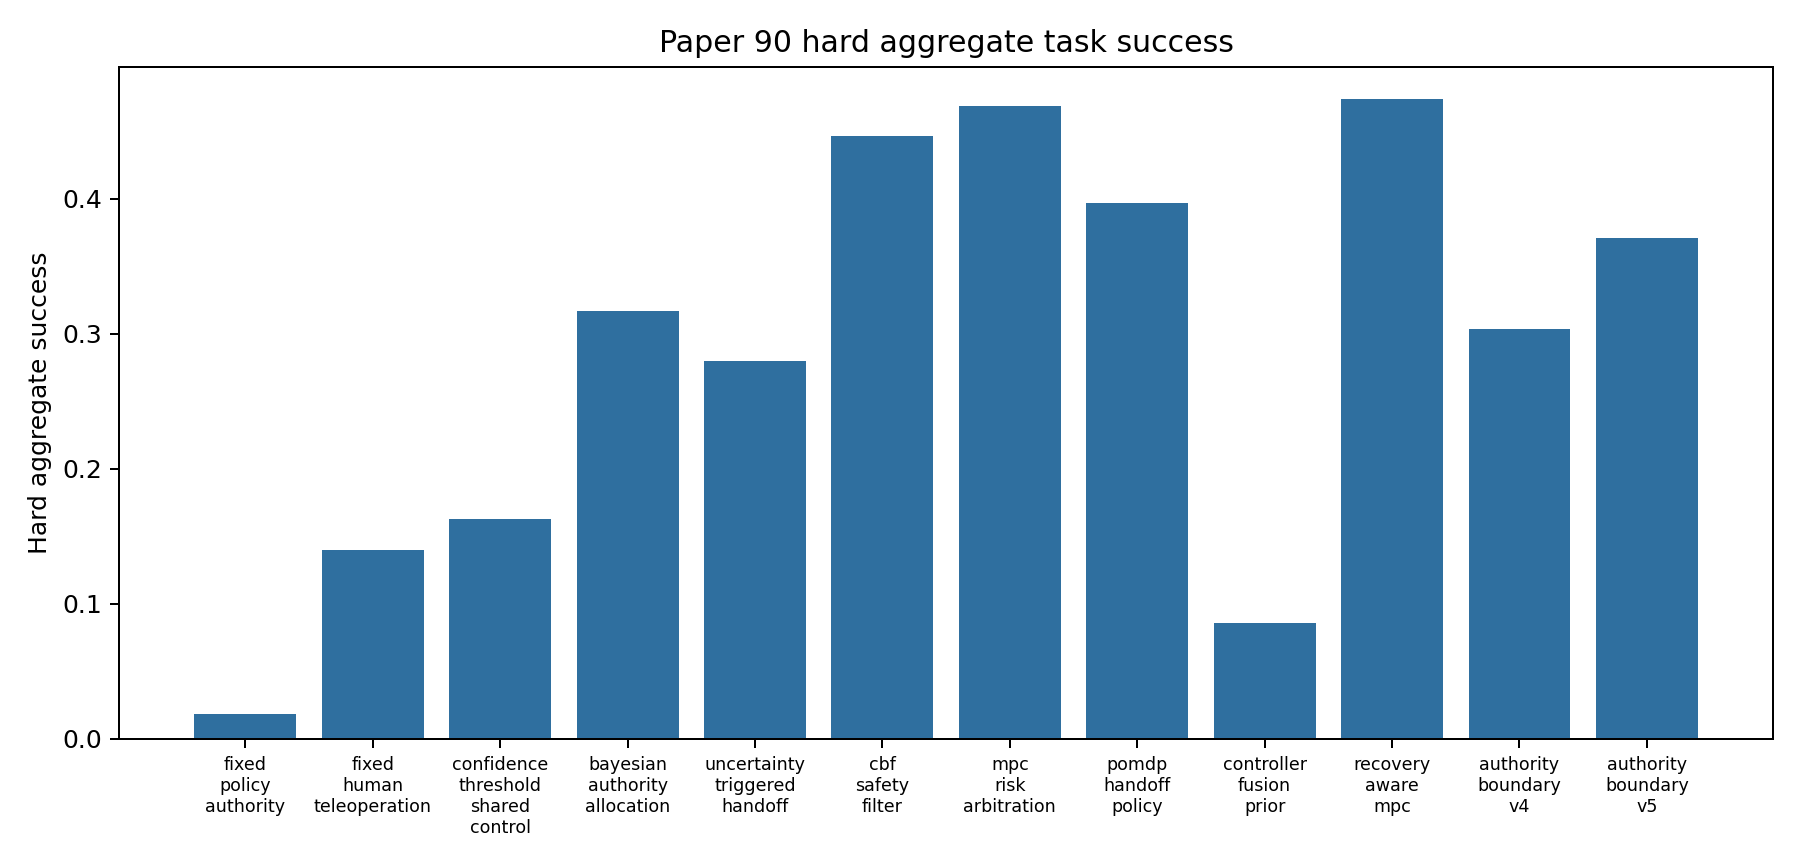
\includegraphics[width=0.95\linewidth]{authority_boundary_hard_success_v5.png}\caption{Hard-aggregate task success.}\end{figure}

\begin{figure}[t]\centering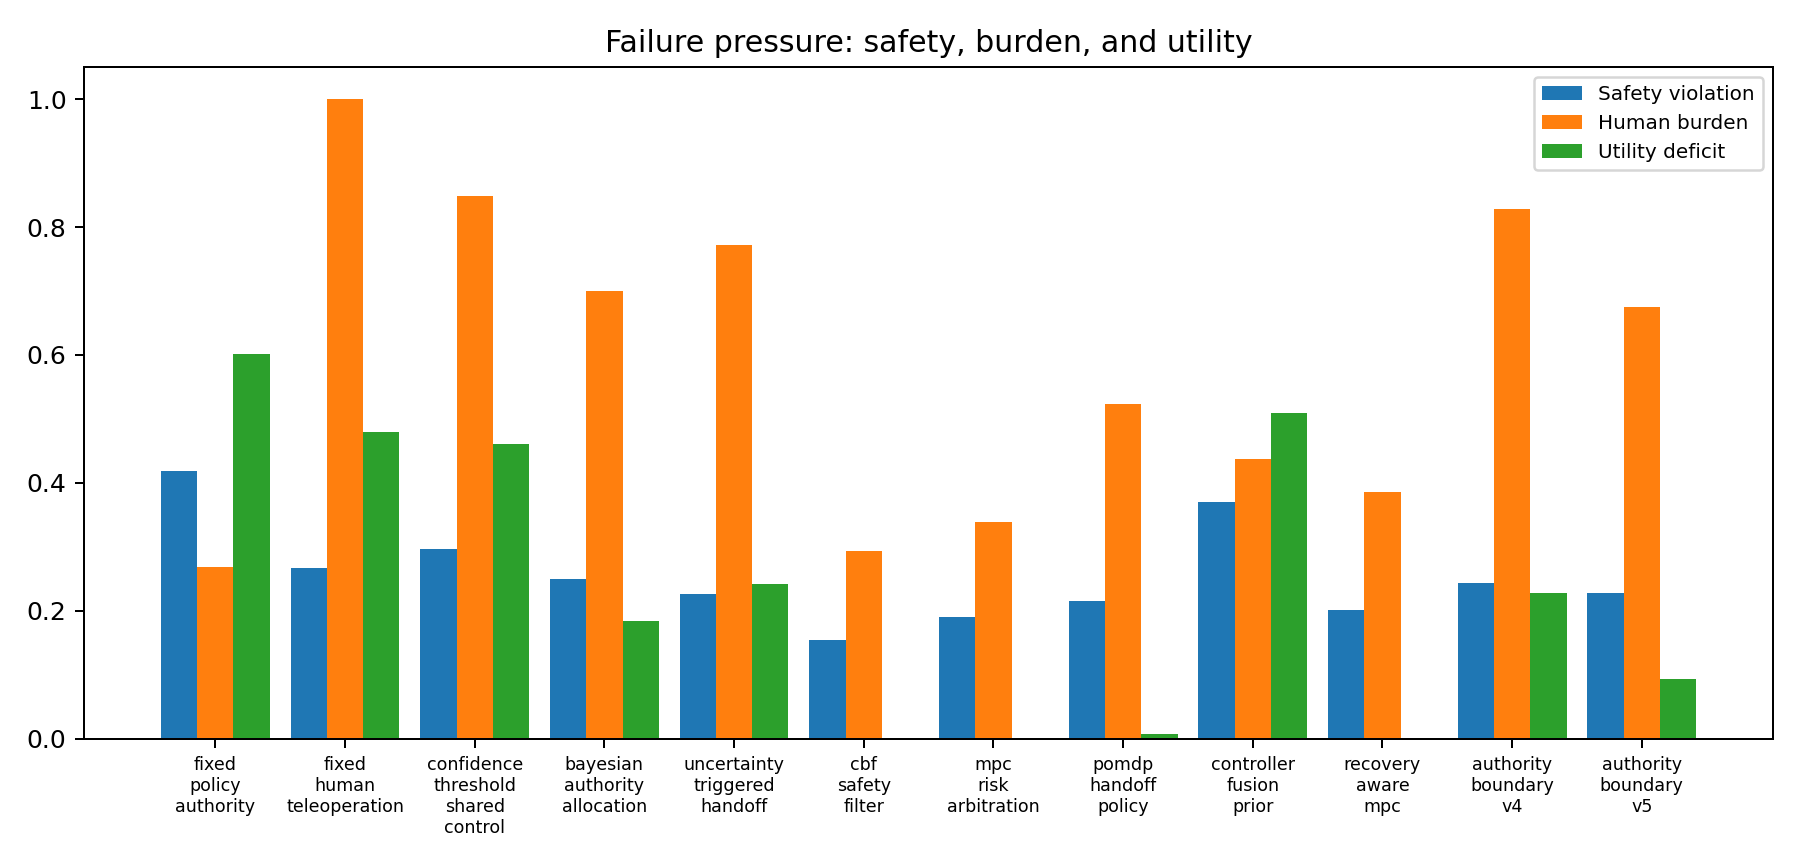
\includegraphics[width=0.95\linewidth]{authority_boundary_failures_v5.png}\caption{Safety, human burden, and utility deficit.}\end{figure}

\section{Split-Level Evidence}

\begin{center}
\scriptsize
\begin{longtable}{p{0.17\linewidth}p{0.25\linewidth}rrrrr}
\caption{Split-level results for the strongest authority baselines and v5.}\label{tab:split}\\
\toprule
Split & Method & Success & Safety & Burden & Regret & Utility\\
\midrule
\endfirsthead
\caption[]{Split-level results for the strongest authority baselines and v5. (continued)}\\
\toprule
Split & Method & Success & Safety & Burden & Regret & Utility\\
\midrule
\endhead
Nominal & Confidence shared & 0.305 $\pm$ 0.014 & 0.228 & 0.754 & 0.375 & -0.195\\
Nominal & Bayesian allocation & 0.463 $\pm$ 0.014 & 0.171 & 0.604 & 0.270 & 0.093\\
Nominal & Uncertainty handoff & 0.408 $\pm$ 0.011 & 0.188 & 0.676 & 0.291 & -0.009\\
Nominal & CBF safety & 0.558 $\pm$ 0.019 & 0.105 & 0.198 & 0.204 & 0.383\\
Nominal & MPC risk & 0.612 $\pm$ 0.014 & 0.142 & 0.244 & 0.181 & 0.409\\
Nominal & POMDP handoff & 0.549 $\pm$ 0.022 & 0.166 & 0.428 & 0.218 & 0.258\\
Nominal & Recovery MPC & 0.609 $\pm$ 0.019 & 0.153 & 0.291 & 0.195 & 0.383\\
Nominal & Authority v5 & 0.512 $\pm$ 0.023 & 0.164 & 0.579 & 0.250 & 0.168\\
Intent ambiguity & Confidence shared & 0.230 $\pm$ 0.009 & 0.247 & 0.834 & 0.412 & -0.340\\
Intent ambiguity & Bayesian allocation & 0.390 $\pm$ 0.014 & 0.200 & 0.684 & 0.306 & -0.057\\
Intent ambiguity & Uncertainty handoff & 0.322 $\pm$ 0.022 & 0.200 & 0.757 & 0.328 & -0.162\\
Intent ambiguity & CBF safety & 0.499 $\pm$ 0.024 & 0.128 & 0.279 & 0.240 & 0.250\\
Intent ambiguity & MPC risk & 0.539 $\pm$ 0.018 & 0.154 & 0.324 & 0.218 & 0.269\\
Intent ambiguity & POMDP handoff & 0.461 $\pm$ 0.018 & 0.176 & 0.508 & 0.255 & 0.103\\
Intent ambiguity & Recovery MPC & 0.553 $\pm$ 0.023 & 0.168 & 0.371 & 0.231 & 0.258\\
Intent ambiguity & Authority v5 & 0.436 $\pm$ 0.030 & 0.168 & 0.660 & 0.286 & 0.029\\
Contact mode & Confidence shared & 0.248 $\pm$ 0.021 & 0.272 & 0.779 & 0.403 & -0.304\\
Contact mode & Bayesian allocation & 0.395 $\pm$ 0.022 & 0.202 & 0.628 & 0.296 & -0.018\\
Contact mode & Uncertainty handoff & 0.368 $\pm$ 0.023 & 0.207 & 0.701 & 0.318 & -0.085\\
Contact mode & CBF safety & 0.520 $\pm$ 0.017 & 0.145 & 0.223 & 0.228 & 0.296\\
Contact mode & MPC risk & 0.537 $\pm$ 0.020 & 0.179 & 0.269 & 0.207 & 0.287\\
Contact mode & POMDP handoff & 0.479 $\pm$ 0.027 & 0.209 & 0.452 & 0.245 & 0.135\\
Contact mode & Recovery MPC & 0.557 $\pm$ 0.020 & 0.183 & 0.316 & 0.221 & 0.288\\
Contact mode & Authority v5 & 0.440 $\pm$ 0.032 & 0.196 & 0.604 & 0.276 & 0.051\\
Human delay & Confidence shared & 0.191 $\pm$ 0.028 & 0.253 & 0.852 & 0.424 & -0.398\\
Human delay & Bayesian allocation & 0.332 $\pm$ 0.022 & 0.188 & 0.701 & 0.318 & -0.122\\
Human delay & Uncertainty handoff & 0.315 $\pm$ 0.029 & 0.215 & 0.775 & 0.340 & -0.194\\
Human delay & CBF safety & 0.488 $\pm$ 0.021 & 0.139 & 0.295 & 0.251 & 0.218\\
Human delay & MPC risk & 0.501 $\pm$ 0.020 & 0.145 & 0.341 & 0.230 & 0.222\\
Human delay & POMDP handoff & 0.440 $\pm$ 0.017 & 0.188 & 0.526 & 0.266 & 0.060\\
Human delay & Recovery MPC & 0.507 $\pm$ 0.016 & 0.173 & 0.389 & 0.243 & 0.194\\
Human delay & Authority v5 & 0.395 $\pm$ 0.013 & 0.201 & 0.677 & 0.298 & -0.046\\
Fragile object & Confidence shared & 0.226 $\pm$ 0.013 & 0.288 & 0.795 & 0.412 & -0.348\\
Fragile object & Bayesian allocation & 0.361 $\pm$ 0.034 & 0.228 & 0.646 & 0.305 & -0.080\\
Fragile object & Uncertainty handoff & 0.327 $\pm$ 0.018 & 0.196 & 0.718 & 0.327 & -0.132\\
Fragile object & CBF safety & 0.499 $\pm$ 0.024 & 0.154 & 0.240 & 0.236 & 0.258\\
Fragile object & MPC risk & 0.527 $\pm$ 0.028 & 0.186 & 0.287 & 0.216 & 0.260\\
Fragile object & POMDP handoff & 0.445 $\pm$ 0.018 & 0.185 & 0.470 & 0.253 & 0.104\\
Fragile object & Recovery MPC & 0.537 $\pm$ 0.016 & 0.177 & 0.333 & 0.229 & 0.260\\
Fragile object & Authority v5 & 0.428 $\pm$ 0.016 & 0.189 & 0.621 & 0.285 & 0.031\\
Authority churn & Confidence shared & 0.160 $\pm$ 0.016 & 0.277 & 0.850 & 0.437 & -0.456\\
Authority churn & Bayesian allocation & 0.346 $\pm$ 0.022 & 0.251 & 0.699 & 0.330 & -0.161\\
Authority churn & Uncertainty handoff & 0.295 $\pm$ 0.024 & 0.215 & 0.773 & 0.352 & -0.226\\
Authority churn & CBF safety & 0.454 $\pm$ 0.021 & 0.143 & 0.295 & 0.262 & 0.169\\
Authority churn & MPC risk & 0.471 $\pm$ 0.017 & 0.183 & 0.340 & 0.241 & 0.155\\
Authority churn & POMDP handoff & 0.418 $\pm$ 0.022 & 0.223 & 0.523 & 0.278 & 0.004\\
Authority churn & Recovery MPC & 0.478 $\pm$ 0.016 & 0.193 & 0.387 & 0.255 & 0.139\\
Authority churn & Authority v5 & 0.377 $\pm$ 0.021 & 0.214 & 0.676 & 0.310 & -0.086\\
Low-signal risk & Confidence shared & 0.145 $\pm$ 0.014 & 0.315 & 0.868 & 0.449 & -0.500\\
Low-signal risk & Bayesian allocation & 0.299 $\pm$ 0.026 & 0.259 & 0.718 & 0.342 & -0.217\\
Low-signal risk & Uncertainty handoff & 0.270 $\pm$ 0.014 & 0.235 & 0.790 & 0.364 & -0.268\\
Low-signal risk & CBF safety & 0.421 $\pm$ 0.024 & 0.153 & 0.312 & 0.273 & 0.126\\
Low-signal risk & MPC risk & 0.448 $\pm$ 0.017 & 0.201 & 0.357 & 0.252 & 0.117\\
Low-signal risk & POMDP handoff & 0.361 $\pm$ 0.018 & 0.232 & 0.541 & 0.289 & -0.063\\
Low-signal risk & Recovery MPC & 0.450 $\pm$ 0.018 & 0.208 & 0.405 & 0.266 & 0.098\\
Low-signal risk & Authority v5 & 0.354 $\pm$ 0.019 & 0.247 & 0.694 & 0.321 & -0.134\\
Combined stress & Confidence shared & 0.119 $\pm$ 0.015 & 0.306 & 0.883 & 0.461 & -0.540\\
Combined stress & Bayesian allocation & 0.260 $\pm$ 0.017 & 0.261 & 0.734 & 0.354 & -0.276\\
Combined stress & Uncertainty handoff & 0.228 $\pm$ 0.018 & 0.258 & 0.807 & 0.375 & -0.344\\
Combined stress & CBF safety & 0.411 $\pm$ 0.027 & 0.167 & 0.329 & 0.285 & 0.088\\
Combined stress & MPC risk & 0.430 $\pm$ 0.010 & 0.192 & 0.374 & 0.263 & 0.085\\
Combined stress & POMDP handoff & 0.365 $\pm$ 0.029 & 0.224 & 0.559 & 0.301 & -0.074\\
Combined stress & Recovery MPC & 0.430 $\pm$ 0.026 & 0.229 & 0.421 & 0.277 & 0.047\\
Combined stress & Authority v5 & 0.326 $\pm$ 0.017 & 0.260 & 0.709 & 0.334 & -0.188\\
\bottomrule
\end{longtable}
\normalsize
\end{center}

\section{Paired Seed Tests}

\begin{center}
\scriptsize
\begin{longtable}{p{0.30\linewidth}p{0.20\linewidth}rrrr}
\caption{Paired seed-level differences for authority v5 minus selected references on the hard aggregate.}\label{tab:paired}\\
\toprule
Reference & Metric & Mean diff & CI95 & Lower95 & Upper95\\
\midrule
\endfirsthead
\caption[]{Paired seed-level differences for authority v5 minus selected references on the hard aggregate. (continued)}\\
\toprule
Reference & Metric & Mean diff & CI95 & Lower95 & Upper95\\
\midrule
\endhead
Recovery MPC & Success & -0.103 & 0.018 & -0.121 & -0.085\\
Recovery MPC & Safety & 0.026 & 0.016 & 0.010 & 0.042\\
Recovery MPC & Burden & 0.289 & 0.001 & 0.288 & 0.289\\
Recovery MPC & Regret & 0.056 & 0.000 & 0.055 & 0.056\\
Recovery MPC & Late & 0.031 & 0.000 & 0.031 & 0.032\\
Recovery MPC & Utility & -0.230 & 0.017 & -0.247 & -0.213\\
CBF safety & Success & -0.076 & 0.012 & -0.087 & -0.064\\
CBF safety & Safety & 0.073 & 0.009 & 0.064 & 0.083\\
CBF safety & Burden & 0.381 & 0.001 & 0.381 & 0.382\\
CBF safety & Regret & 0.048 & 0.000 & 0.048 & 0.049\\
CBF safety & Late & 0.012 & 0.000 & 0.011 & 0.012\\
CBF safety & Utility & -0.254 & 0.010 & -0.264 & -0.244\\
MPC risk & Success & -0.098 & 0.016 & -0.114 & -0.082\\
MPC risk & Safety & 0.037 & 0.011 & 0.025 & 0.048\\
MPC risk & Burden & 0.336 & 0.001 & 0.335 & 0.336\\
MPC risk & Regret & 0.070 & 0.000 & 0.069 & 0.070\\
MPC risk & Late & 0.027 & 0.000 & 0.027 & 0.027\\
MPC risk & Utility & -0.249 & 0.015 & -0.263 & -0.234\\
Authority v4 & Success & 0.067 & 0.016 & 0.051 & 0.083\\
Authority v4 & Safety & -0.016 & 0.014 & -0.030 & -0.002\\
Authority v4 & Burden & -0.154 & 0.000 & -0.154 & -0.153\\
Authority v4 & Regret & -0.036 & 0.000 & -0.036 & -0.035\\
Authority v4 & Late & -0.015 & 0.000 & -0.015 & -0.015\\
Authority v4 & Utility & 0.135 & 0.020 & 0.114 & 0.155\\
\bottomrule
\end{longtable}
\normalsize
\end{center}

\section{Complete Split Paired Checks}

Table~\ref{tab:splitpaired} reports the split-level paired comparisons that hostile reviewers would otherwise ask for after seeing only the hard aggregate.

\begin{center}
\tiny
\begin{longtable}{p{0.17\linewidth}p{0.25\linewidth}p{0.16\linewidth}rrr}
\caption{Complete split-level paired checks for success, safety, burden, and utility.}\label{tab:splitpaired}\\
\toprule
Split & Reference & Metric & Mean diff & Lower95 & Upper95\\
\midrule
\endfirsthead
\caption[]{Complete split-level paired checks for success, safety, burden, and utility. (continued)}\\
\toprule
Split & Reference & Metric & Mean diff & Lower95 & Upper95\\
\midrule
\endhead
Authority churn & Authority v4 & Burden & -0.154 & -0.154 & -0.153\\
Authority churn & Authority v4 & Utility & 0.126 & 0.094 & 0.158\\
Authority churn & Authority v4 & Safety & -0.003 & -0.015 & 0.009\\
Authority churn & Authority v4 & Success & 0.067 & 0.036 & 0.097\\
Authority churn & Bayesian allocation & Burden & -0.023 & -0.024 & -0.022\\
Authority churn & Bayesian allocation & Utility & 0.075 & 0.027 & 0.122\\
Authority churn & Bayesian allocation & Safety & -0.037 & -0.062 & -0.013\\
Authority churn & Bayesian allocation & Success & 0.031 & -0.009 & 0.070\\
Authority churn & CBF safety & Burden & 0.381 & 0.380 & 0.382\\
Authority churn & CBF safety & Utility & -0.255 & -0.296 & -0.213\\
Authority churn & CBF safety & Safety & 0.071 & 0.051 & 0.090\\
Authority churn & CBF safety & Success & -0.078 & -0.117 & -0.039\\
Authority churn & MPC risk & Burden & 0.336 & 0.335 & 0.338\\
Authority churn & MPC risk & Utility & -0.241 & -0.270 & -0.212\\
Authority churn & MPC risk & Safety & 0.030 & 0.008 & 0.052\\
Authority churn & MPC risk & Success & -0.094 & -0.127 & -0.061\\
Authority churn & POMDP handoff & Burden & 0.153 & 0.152 & 0.154\\
Authority churn & POMDP handoff & Utility & -0.089 & -0.118 & -0.061\\
Authority churn & POMDP handoff & Safety & -0.010 & -0.027 & 0.007\\
Authority churn & POMDP handoff & Success & -0.042 & -0.067 & -0.016\\
Authority churn & Recovery MPC & Burden & 0.289 & 0.289 & 0.290\\
Authority churn & Recovery MPC & Utility & -0.225 & -0.255 & -0.196\\
Authority churn & Recovery MPC & Safety & 0.020 & 0.003 & 0.038\\
Authority churn & Recovery MPC & Success & -0.101 & -0.127 & -0.075\\
Authority churn & Uncertainty handoff & Burden & -0.097 & -0.098 & -0.096\\
Authority churn & Uncertainty handoff & Utility & 0.140 & 0.097 & 0.183\\
Authority churn & Uncertainty handoff & Safety & -0.001 & -0.026 & 0.024\\
Authority churn & Uncertainty handoff & Success & 0.082 & 0.048 & 0.115\\
Combined stress & Authority v4 & Burden & -0.154 & -0.155 & -0.153\\
Combined stress & Authority v4 & Utility & 0.120 & 0.077 & 0.163\\
Combined stress & Authority v4 & Safety & 0.003 & -0.039 & 0.046\\
Combined stress & Authority v4 & Success & 0.064 & 0.041 & 0.087\\
Combined stress & Bayesian allocation & Burden & -0.025 & -0.026 & -0.024\\
Combined stress & Bayesian allocation & Utility & 0.088 & 0.061 & 0.116\\
Combined stress & Bayesian allocation & Safety & -0.001 & -0.041 & 0.039\\
Combined stress & Bayesian allocation & Success & 0.066 & 0.037 & 0.096\\
Combined stress & CBF safety & Burden & 0.381 & 0.379 & 0.382\\
Combined stress & CBF safety & Utility & -0.276 & -0.314 & -0.238\\
Combined stress & CBF safety & Safety & 0.093 & 0.069 & 0.116\\
Combined stress & CBF safety & Success & -0.085 & -0.120 & -0.050\\
Combined stress & MPC risk & Burden & 0.336 & 0.334 & 0.337\\
Combined stress & MPC risk & Utility & -0.273 & -0.294 & -0.253\\
Combined stress & MPC risk & Safety & 0.068 & 0.037 & 0.098\\
Combined stress & MPC risk & Success & -0.104 & -0.123 & -0.084\\
Combined stress & POMDP handoff & Burden & 0.151 & 0.150 & 0.151\\
Combined stress & POMDP handoff & Utility & -0.114 & -0.147 & -0.082\\
Combined stress & POMDP handoff & Safety & 0.036 & 0.003 & 0.069\\
Combined stress & POMDP handoff & Success & -0.039 & -0.073 & -0.004\\
Combined stress & Recovery MPC & Burden & 0.288 & 0.287 & 0.289\\
Combined stress & Recovery MPC & Utility & -0.235 & -0.279 & -0.191\\
Combined stress & Recovery MPC & Safety & 0.031 & 0.006 & 0.057\\
Combined stress & Recovery MPC & Success & -0.104 & -0.141 & -0.067\\
Combined stress & Uncertainty handoff & Burden & -0.097 & -0.098 & -0.096\\
Combined stress & Uncertainty handoff & Utility & 0.155 & 0.122 & 0.189\\
Combined stress & Uncertainty handoff & Safety & 0.002 & -0.026 & 0.029\\
Combined stress & Uncertainty handoff & Success & 0.098 & 0.067 & 0.130\\
Contact mode & Authority v4 & Burden & -0.154 & -0.155 & -0.152\\
Contact mode & Authority v4 & Utility & 0.148 & 0.118 & 0.178\\
Contact mode & Authority v4 & Safety & -0.029 & -0.060 & 0.003\\
Contact mode & Authority v4 & Success & 0.073 & 0.035 & 0.111\\
Contact mode & Bayesian allocation & Burden & -0.024 & -0.024 & -0.023\\
Contact mode & Bayesian allocation & Utility & 0.069 & 0.030 & 0.109\\
Contact mode & Bayesian allocation & Safety & -0.006 & -0.025 & 0.013\\
Contact mode & Bayesian allocation & Success & 0.045 & 0.006 & 0.084\\
Contact mode & CBF safety & Burden & 0.381 & 0.380 & 0.383\\
Contact mode & CBF safety & Utility & -0.244 & -0.268 & -0.221\\
Contact mode & CBF safety & Safety & 0.051 & 0.013 & 0.089\\
Contact mode & CBF safety & Success & -0.080 & -0.108 & -0.052\\
Contact mode & MPC risk & Burden & 0.335 & 0.333 & 0.337\\
Contact mode & MPC risk & Utility & -0.236 & -0.271 & -0.201\\
Contact mode & MPC risk & Safety & 0.018 & -0.007 & 0.043\\
Contact mode & MPC risk & Success & -0.097 & -0.137 & -0.058\\
Contact mode & POMDP handoff & Burden & 0.152 & 0.150 & 0.154\\
Contact mode & POMDP handoff & Utility & -0.084 & -0.123 & -0.045\\
Contact mode & POMDP handoff & Safety & -0.013 & -0.036 & 0.010\\
Contact mode & POMDP handoff & Success & -0.039 & -0.069 & -0.008\\
Contact mode & Recovery MPC & Burden & 0.288 & 0.288 & 0.289\\
Contact mode & Recovery MPC & Utility & -0.236 & -0.275 & -0.198\\
Contact mode & Recovery MPC & Safety & 0.014 & -0.012 & 0.039\\
Contact mode & Recovery MPC & Success & -0.117 & -0.155 & -0.078\\
Contact mode & Uncertainty handoff & Burden & -0.097 & -0.098 & -0.096\\
Contact mode & Uncertainty handoff & Utility & 0.137 & 0.088 & 0.186\\
Contact mode & Uncertainty handoff & Safety & -0.011 & -0.033 & 0.011\\
Contact mode & Uncertainty handoff & Success & 0.072 & 0.022 & 0.122\\
Fragile object & Authority v4 & Burden & -0.154 & -0.155 & -0.153\\
Fragile object & Authority v4 & Utility & 0.154 & 0.128 & 0.180\\
Fragile object & Authority v4 & Safety & -0.053 & -0.074 & -0.032\\
Fragile object & Authority v4 & Success & 0.064 & 0.043 & 0.084\\
Fragile object & Bayesian allocation & Burden & -0.025 & -0.026 & -0.024\\
Fragile object & Bayesian allocation & Utility & 0.112 & 0.079 & 0.144\\
Fragile object & Bayesian allocation & Safety & -0.040 & -0.069 & -0.010\\
Fragile object & Bayesian allocation & Success & 0.066 & 0.039 & 0.093\\
Fragile object & CBF safety & Burden & 0.381 & 0.380 & 0.382\\
Fragile object & CBF safety & Utility & -0.226 & -0.247 & -0.206\\
Fragile object & CBF safety & Safety & 0.035 & 0.006 & 0.064\\
Fragile object & CBF safety & Success & -0.071 & -0.089 & -0.054\\
Fragile object & MPC risk & Burden & 0.335 & 0.333 & 0.336\\
Fragile object & MPC risk & Utility & -0.229 & -0.266 & -0.191\\
Fragile object & MPC risk & Safety & 0.003 & -0.023 & 0.029\\
Fragile object & MPC risk & Success & -0.099 & -0.137 & -0.062\\
Fragile object & POMDP handoff & Burden & 0.151 & 0.150 & 0.152\\
Fragile object & POMDP handoff & Utility & -0.073 & -0.100 & -0.045\\
Fragile object & POMDP handoff & Safety & 0.003 & -0.022 & 0.028\\
Fragile object & POMDP handoff & Success & -0.017 & -0.040 & 0.005\\
Fragile object & Recovery MPC & Burden & 0.288 & 0.287 & 0.289\\
Fragile object & Recovery MPC & Utility & -0.228 & -0.257 & -0.199\\
Fragile object & Recovery MPC & Safety & 0.012 & -0.022 & 0.046\\
Fragile object & Recovery MPC & Success & -0.109 & -0.132 & -0.087\\
Fragile object & Uncertainty handoff & Burden & -0.097 & -0.098 & -0.095\\
Fragile object & Uncertainty handoff & Utility & 0.164 & 0.137 & 0.191\\
Fragile object & Uncertainty handoff & Safety & -0.008 & -0.030 & 0.014\\
Fragile object & Uncertainty handoff & Success & 0.101 & 0.078 & 0.124\\
Human delay & Authority v4 & Burden & -0.154 & -0.155 & -0.152\\
Human delay & Authority v4 & Utility & 0.136 & 0.102 & 0.171\\
Human delay & Authority v4 & Safety & 0.010 & -0.023 & 0.044\\
Human delay & Authority v4 & Success & 0.085 & 0.059 & 0.112\\
Human delay & Bayesian allocation & Burden & -0.024 & -0.025 & -0.023\\
Human delay & Bayesian allocation & Utility & 0.076 & 0.037 & 0.114\\
Human delay & Bayesian allocation & Safety & 0.013 & -0.012 & 0.038\\
Human delay & Bayesian allocation & Success & 0.062 & 0.031 & 0.094\\
Human delay & CBF safety & Burden & 0.381 & 0.380 & 0.382\\
Human delay & CBF safety & Utility & -0.264 & -0.295 & -0.234\\
Human delay & CBF safety & Safety & 0.061 & 0.034 & 0.089\\
Human delay & CBF safety & Success & -0.093 & -0.117 & -0.070\\
Human delay & MPC risk & Burden & 0.336 & 0.334 & 0.337\\
Human delay & MPC risk & Utility & -0.268 & -0.286 & -0.251\\
Human delay & MPC risk & Safety & 0.056 & 0.027 & 0.084\\
Human delay & MPC risk & Success & -0.106 & -0.125 & -0.088\\
Human delay & POMDP handoff & Burden & 0.151 & 0.150 & 0.152\\
Human delay & POMDP handoff & Utility & -0.106 & -0.133 & -0.080\\
Human delay & POMDP handoff & Safety & 0.013 & -0.005 & 0.030\\
Human delay & POMDP handoff & Success & -0.045 & -0.067 & -0.023\\
Human delay & Recovery MPC & Burden & 0.288 & 0.287 & 0.290\\
Human delay & Recovery MPC & Utility & -0.240 & -0.273 & -0.207\\
Human delay & Recovery MPC & Safety & 0.027 & 0.003 & 0.051\\
Human delay & Recovery MPC & Success & -0.112 & -0.135 & -0.089\\
Human delay & Uncertainty handoff & Burden & -0.098 & -0.099 & -0.096\\
Human delay & Uncertainty handoff & Utility & 0.147 & 0.110 & 0.184\\
Human delay & Uncertainty handoff & Safety & -0.014 & -0.030 & 0.002\\
Human delay & Uncertainty handoff & Success & 0.080 & 0.049 & 0.111\\
Intent ambiguity & Authority v4 & Burden & -0.154 & -0.155 & -0.152\\
Intent ambiguity & Authority v4 & Utility & 0.145 & 0.115 & 0.175\\
Intent ambiguity & Authority v4 & Safety & -0.032 & -0.054 & -0.010\\
Intent ambiguity & Authority v4 & Success & 0.068 & 0.045 & 0.091\\
Intent ambiguity & Bayesian allocation & Burden & -0.024 & -0.025 & -0.023\\
Intent ambiguity & Bayesian allocation & Utility & 0.086 & 0.050 & 0.123\\
Intent ambiguity & Bayesian allocation & Safety & -0.032 & -0.047 & -0.016\\
Intent ambiguity & Bayesian allocation & Success & 0.046 & 0.010 & 0.082\\
Intent ambiguity & CBF safety & Burden & 0.381 & 0.380 & 0.382\\
Intent ambiguity & CBF safety & Utility & -0.221 & -0.253 & -0.188\\
Intent ambiguity & CBF safety & Safety & 0.041 & 0.025 & 0.056\\
Intent ambiguity & CBF safety & Success & -0.063 & -0.100 & -0.026\\
Intent ambiguity & MPC risk & Burden & 0.336 & 0.335 & 0.337\\
Intent ambiguity & MPC risk & Utility & -0.240 & -0.280 & -0.199\\
Intent ambiguity & MPC risk & Safety & 0.015 & 0.001 & 0.028\\
Intent ambiguity & MPC risk & Success & -0.103 & -0.139 & -0.067\\
Intent ambiguity & POMDP handoff & Burden & 0.151 & 0.151 & 0.152\\
Intent ambiguity & POMDP handoff & Utility & -0.073 & -0.109 & -0.038\\
Intent ambiguity & POMDP handoff & Safety & -0.008 & -0.031 & 0.015\\
Intent ambiguity & POMDP handoff & Success & -0.025 & -0.053 & 0.003\\
Intent ambiguity & Recovery MPC & Burden & 0.288 & 0.287 & 0.290\\
Intent ambiguity & Recovery MPC & Utility & -0.228 & -0.275 & -0.182\\
Intent ambiguity & Recovery MPC & Safety & -0.000 & -0.020 & 0.020\\
Intent ambiguity & Recovery MPC & Success & -0.117 & -0.155 & -0.080\\
Intent ambiguity & Uncertainty handoff & Burden & -0.097 & -0.098 & -0.096\\
Intent ambiguity & Uncertainty handoff & Utility & 0.191 & 0.162 & 0.221\\
Intent ambiguity & Uncertainty handoff & Safety & -0.032 & -0.053 & -0.011\\
Intent ambiguity & Uncertainty handoff & Success & 0.114 & 0.089 & 0.138\\
Low-signal risk & Authority v4 & Burden & -0.153 & -0.154 & -0.152\\
Low-signal risk & Authority v4 & Utility & 0.139 & 0.107 & 0.170\\
Low-signal risk & Authority v4 & Safety & -0.010 & -0.042 & 0.021\\
Low-signal risk & Authority v4 & Success & 0.075 & 0.049 & 0.101\\
Low-signal risk & Bayesian allocation & Burden & -0.024 & -0.025 & -0.023\\
Low-signal risk & Bayesian allocation & Utility & 0.083 & 0.045 & 0.121\\
Low-signal risk & Bayesian allocation & Safety & -0.012 & -0.040 & 0.016\\
Low-signal risk & Bayesian allocation & Success & 0.055 & 0.020 & 0.089\\
Low-signal risk & CBF safety & Burden & 0.382 & 0.381 & 0.383\\
Low-signal risk & CBF safety & Utility & -0.260 & -0.298 & -0.222\\
Low-signal risk & CBF safety & Safety & 0.095 & 0.081 & 0.108\\
Low-signal risk & CBF safety & Success & -0.068 & -0.102 & -0.034\\
Low-signal risk & MPC risk & Burden & 0.337 & 0.336 & 0.338\\
Low-signal risk & MPC risk & Utility & -0.252 & -0.275 & -0.229\\
Low-signal risk & MPC risk & Safety & 0.046 & 0.028 & 0.065\\
Low-signal risk & MPC risk & Success & -0.095 & -0.115 & -0.074\\
Low-signal risk & POMDP handoff & Burden & 0.153 & 0.152 & 0.154\\
Low-signal risk & POMDP handoff & Utility & -0.071 & -0.100 & -0.043\\
Low-signal risk & POMDP handoff & Safety & 0.016 & -0.009 & 0.041\\
Low-signal risk & POMDP handoff & Success & -0.007 & -0.031 & 0.016\\
Low-signal risk & Recovery MPC & Burden & 0.289 & 0.288 & 0.290\\
Low-signal risk & Recovery MPC & Utility & -0.233 & -0.251 & -0.214\\
Low-signal risk & Recovery MPC & Safety & 0.040 & 0.023 & 0.056\\
Low-signal risk & Recovery MPC & Success & -0.096 & -0.115 & -0.078\\
Low-signal risk & Uncertainty handoff & Burden & -0.096 & -0.097 & -0.096\\
Low-signal risk & Uncertainty handoff & Utility & 0.134 & 0.104 & 0.164\\
Low-signal risk & Uncertainty handoff & Safety & 0.012 & -0.014 & 0.038\\
Low-signal risk & Uncertainty handoff & Success & 0.083 & 0.059 & 0.108\\
Nominal & Authority v4 & Burden & -0.154 & -0.155 & -0.153\\
Nominal & Authority v4 & Utility & 0.145 & 0.108 & 0.183\\
Nominal & Authority v4 & Safety & -0.019 & -0.042 & 0.004\\
Nominal & Authority v4 & Success & 0.077 & 0.039 & 0.114\\
Nominal & Bayesian allocation & Burden & -0.024 & -0.026 & -0.023\\
Nominal & Bayesian allocation & Utility & 0.075 & 0.053 & 0.097\\
Nominal & Bayesian allocation & Safety & -0.007 & -0.029 & 0.014\\
Nominal & Bayesian allocation & Success & 0.049 & 0.034 & 0.065\\
Nominal & CBF safety & Burden & 0.382 & 0.381 & 0.383\\
Nominal & CBF safety & Utility & -0.214 & -0.242 & -0.187\\
Nominal & CBF safety & Safety & 0.058 & 0.042 & 0.075\\
Nominal & CBF safety & Success & -0.045 & -0.075 & -0.015\\
Nominal & MPC risk & Burden & 0.335 & 0.334 & 0.337\\
Nominal & MPC risk & Utility & -0.241 & -0.269 & -0.212\\
Nominal & MPC risk & Safety & 0.022 & -0.004 & 0.048\\
Nominal & MPC risk & Success & -0.099 & -0.125 & -0.074\\
Nominal & POMDP handoff & Burden & 0.152 & 0.151 & 0.153\\
Nominal & POMDP handoff & Utility & -0.089 & -0.121 & -0.058\\
Nominal & POMDP handoff & Safety & -0.002 & -0.017 & 0.013\\
Nominal & POMDP handoff & Success & -0.037 & -0.065 & -0.009\\
Nominal & Recovery MPC & Burden & 0.288 & 0.287 & 0.290\\
Nominal & Recovery MPC & Utility & -0.214 & -0.255 & -0.174\\
Nominal & Recovery MPC & Safety & 0.010 & -0.009 & 0.030\\
Nominal & Recovery MPC & Success & -0.097 & -0.131 & -0.063\\
Nominal & Uncertainty handoff & Burden & -0.097 & -0.098 & -0.096\\
Nominal & Uncertainty handoff & Utility & 0.178 & 0.146 & 0.210\\
Nominal & Uncertainty handoff & Safety & -0.024 & -0.041 & -0.008\\
Nominal & Uncertainty handoff & Success & 0.105 & 0.077 & 0.132\\
\bottomrule
\end{longtable}
\normalsize
\end{center}

\section{Ablations}

The mechanism gate fails because simpler safety-only and MPC-only variants beat the full model on the combined stress utility target.

\begin{center}
\scriptsize
\begin{longtable}{p{0.16\linewidth}p{0.30\linewidth}rrrrr}
\caption{Mechanism ablations. The full method must beat removals rather than benefit from deletion.}\label{tab:ablation}\\
\toprule
Split & Ablation & Success & Safety & Burden & Regret & Utility\\
\midrule
\endfirsthead
\caption[]{Mechanism ablations. The full method must beat removals rather than benefit from deletion. (continued)}\\
\toprule
Split & Ablation & Success & Safety & Burden & Regret & Utility\\
\midrule
\endhead
Combined stress & Confidence only & 0.122 $\pm$ 0.017 & 0.310 & 0.844 & 0.467 & -0.529\\
Combined stress & Full authority v5 & 0.312 $\pm$ 0.020 & 0.220 & 0.709 & 0.333 & -0.177\\
Combined stress & - boundary uncertainty & 0.300 $\pm$ 0.017 & 0.282 & 0.682 & 0.368 & -0.236\\
Combined stress & - consequence risk & 0.254 $\pm$ 0.020 & 0.317 & 0.683 & 0.393 & -0.308\\
Combined stress & - handoff hysteresis & 0.335 $\pm$ 0.030 & 0.239 & 0.729 & 0.341 & -0.197\\
Combined stress & - human burden & 0.338 $\pm$ 0.020 & 0.261 & 0.898 & 0.321 & -0.225\\
Combined stress & - intent ambiguity & 0.370 $\pm$ 0.028 & 0.257 & 0.518 & 0.298 & -0.071\\
Combined stress & - recovery feasibility & 0.298 $\pm$ 0.018 & 0.245 & 0.690 & 0.355 & -0.218\\
Combined stress & MPC only & 0.418 $\pm$ 0.019 & 0.205 & 0.383 & 0.276 & 0.061\\
Combined stress & Safety only & 0.404 $\pm$ 0.024 & 0.168 & 0.328 & 0.286 & 0.079\\
Low-signal risk & Confidence only & 0.151 $\pm$ 0.014 & 0.334 & 0.827 & 0.454 & -0.496\\
Low-signal risk & Full authority v5 & 0.345 $\pm$ 0.031 & 0.249 & 0.693 & 0.322 & -0.144\\
Low-signal risk & - boundary uncertainty & 0.338 $\pm$ 0.017 & 0.270 & 0.665 & 0.356 & -0.172\\
Low-signal risk & - consequence risk & 0.294 $\pm$ 0.012 & 0.307 & 0.666 & 0.381 & -0.243\\
Low-signal risk & - handoff hysteresis & 0.364 $\pm$ 0.028 & 0.234 & 0.713 & 0.329 & -0.146\\
Low-signal risk & - human burden & 0.335 $\pm$ 0.022 & 0.254 & 0.882 & 0.309 & -0.206\\
Low-signal risk & - intent ambiguity & 0.401 $\pm$ 0.028 & 0.237 & 0.502 & 0.287 & -0.009\\
Low-signal risk & - recovery feasibility & 0.299 $\pm$ 0.028 & 0.240 & 0.672 & 0.343 & -0.195\\
Low-signal risk & MPC only & 0.442 $\pm$ 0.035 & 0.208 & 0.367 & 0.264 & 0.101\\
Low-signal risk & Safety only & 0.446 $\pm$ 0.026 & 0.168 & 0.311 & 0.274 & 0.141\\
\bottomrule
\end{longtable}
\normalsize
\end{center}

\begin{figure}[t]\centering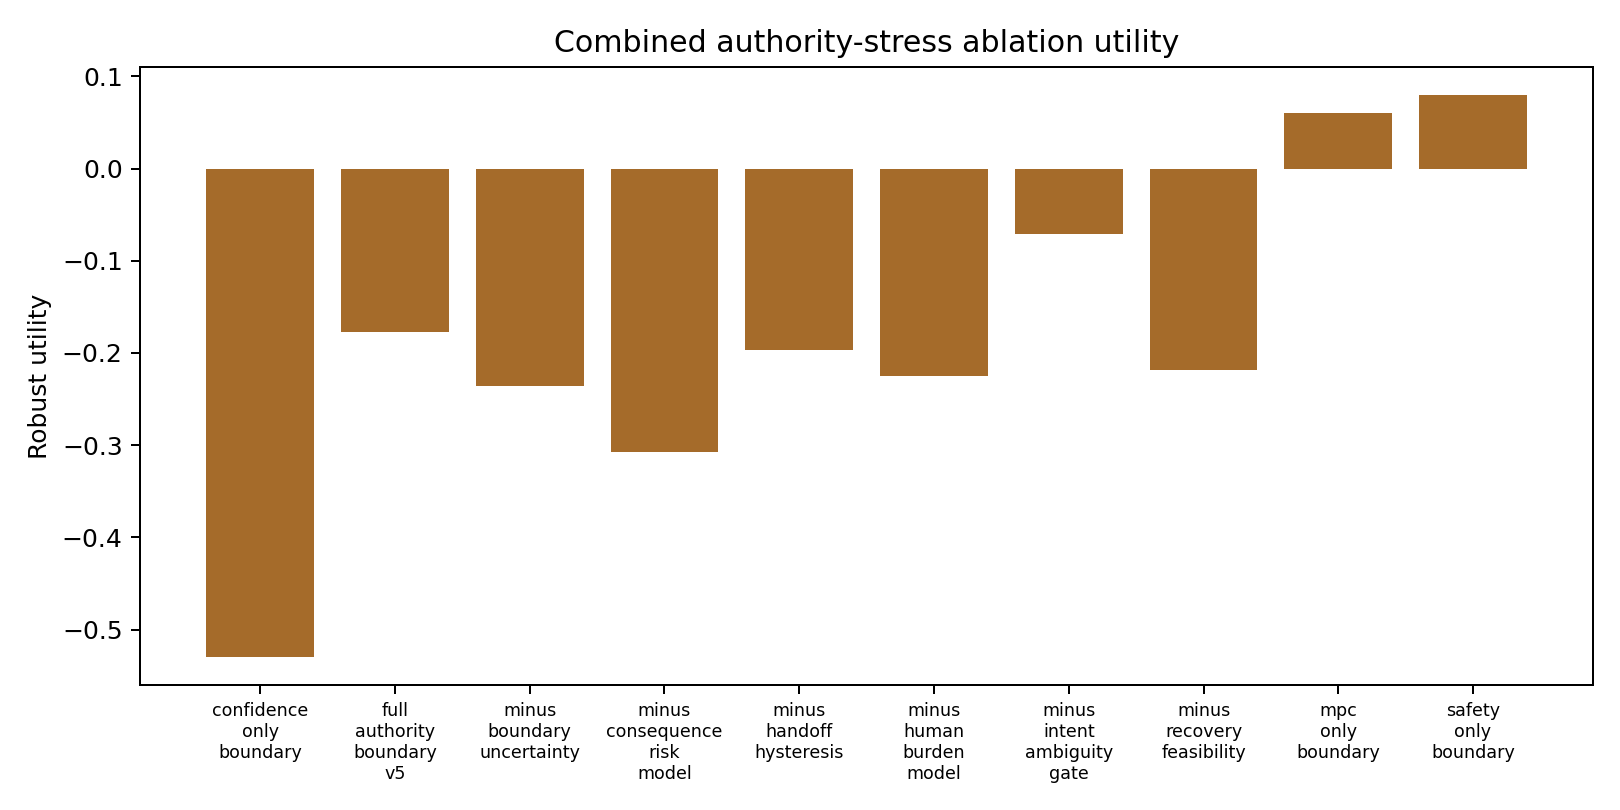
\includegraphics[width=0.95\linewidth]{authority_boundary_ablation_v5.png}\caption{Ablation robust utility on combined authority stress.}\end{figure}

\section{Stress Tests}

\begin{center}
\tiny
\begin{longtable}{p{0.17\linewidth}rp{0.23\linewidth}rrrrr}
\caption{Full stress sweep over six axes and six levels.}\label{tab:stress}\\
\toprule
Axis & Level & Method & Succ. & Safety & Burden & Regret & Utility\\
\midrule
\endfirsthead
\caption[]{Full stress sweep over six axes and six levels. (continued)}\\
\toprule
Axis & Level & Method & Succ. & Safety & Burden & Regret & Utility\\
\midrule
\endhead
authority churn & 0.00 & Authority v5 & 0.313 & 0.229 & 0.709 & 0.326 & -0.169\\
authority churn & 0.00 & Bayesian allocation & 0.261 & 0.244 & 0.734 & 0.345 & -0.252\\
authority churn & 0.00 & CBF safety & 0.416 & 0.170 & 0.327 & 0.276 & 0.104\\
authority churn & 0.00 & Confidence shared & 0.138 & 0.322 & 0.884 & 0.453 & -0.517\\
authority churn & 0.00 & MPC risk & 0.458 & 0.181 & 0.373 & 0.255 & 0.134\\
authority churn & 0.00 & POMDP handoff & 0.382 & 0.223 & 0.557 & 0.293 & -0.043\\
authority churn & 0.00 & Recovery MPC & 0.444 & 0.203 & 0.421 & 0.270 & 0.090\\
authority churn & 0.20 & Authority v5 & 0.313 & 0.266 & 0.709 & 0.330 & -0.198\\
authority churn & 0.20 & Bayesian allocation & 0.262 & 0.257 & 0.733 & 0.350 & -0.265\\
authority churn & 0.20 & CBF safety & 0.403 & 0.173 & 0.328 & 0.281 & 0.082\\
authority churn & 0.20 & Confidence shared & 0.136 & 0.331 & 0.883 & 0.457 & -0.532\\
authority churn & 0.20 & MPC risk & 0.432 & 0.210 & 0.374 & 0.259 & 0.084\\
authority churn & 0.20 & POMDP handoff & 0.346 & 0.217 & 0.558 & 0.297 & -0.082\\
authority churn & 0.20 & Recovery MPC & 0.417 & 0.218 & 0.421 & 0.274 & 0.047\\
authority churn & 0.40 & Authority v5 & 0.321 & 0.238 & 0.709 & 0.334 & -0.181\\
authority churn & 0.40 & Bayesian allocation & 0.270 & 0.254 & 0.734 & 0.354 & -0.262\\
authority churn & 0.40 & CBF safety & 0.405 & 0.163 & 0.329 & 0.285 & 0.083\\
authority churn & 0.40 & Confidence shared & 0.108 & 0.344 & 0.884 & 0.462 & -0.575\\
authority churn & 0.40 & MPC risk & 0.408 & 0.202 & 0.375 & 0.264 & 0.057\\
authority churn & 0.40 & POMDP handoff & 0.377 & 0.230 & 0.558 & 0.302 & -0.066\\
authority churn & 0.40 & Recovery MPC & 0.455 & 0.223 & 0.421 & 0.278 & 0.075\\
authority churn & 0.60 & Authority v5 & 0.335 & 0.238 & 0.709 & 0.339 & -0.174\\
authority churn & 0.60 & Bayesian allocation & 0.255 & 0.270 & 0.734 & 0.359 & -0.294\\
authority churn & 0.60 & CBF safety & 0.372 & 0.166 & 0.327 & 0.290 & 0.043\\
authority churn & 0.60 & Confidence shared & 0.114 & 0.324 & 0.883 & 0.467 & -0.564\\
authority churn & 0.60 & MPC risk & 0.426 & 0.212 & 0.373 & 0.269 & 0.061\\
authority churn & 0.60 & POMDP handoff & 0.336 & 0.253 & 0.558 & 0.306 & -0.128\\
authority churn & 0.60 & Recovery MPC & 0.392 & 0.214 & 0.421 & 0.283 & 0.010\\
authority churn & 0.80 & Authority v5 & 0.325 & 0.252 & 0.709 & 0.344 & -0.199\\
authority churn & 0.80 & Bayesian allocation & 0.249 & 0.261 & 0.733 & 0.364 & -0.302\\
authority churn & 0.80 & CBF safety & 0.373 & 0.184 & 0.328 & 0.294 & 0.025\\
authority churn & 0.80 & Confidence shared & 0.107 & 0.287 & 0.884 & 0.472 & -0.556\\
authority churn & 0.80 & MPC risk & 0.426 & 0.214 & 0.374 & 0.274 & 0.053\\
authority churn & 0.80 & POMDP handoff & 0.341 & 0.242 & 0.558 & 0.312 & -0.124\\
authority churn & 0.80 & Recovery MPC & 0.411 & 0.214 & 0.421 & 0.287 & 0.022\\
authority churn & 1.00 & Authority v5 & 0.311 & 0.279 & 0.709 & 0.345 & -0.232\\
authority churn & 1.00 & Bayesian allocation & 0.253 & 0.290 & 0.733 & 0.366 & -0.318\\
authority churn & 1.00 & CBF safety & 0.390 & 0.170 & 0.328 & 0.296 & 0.048\\
authority churn & 1.00 & Confidence shared & 0.116 & 0.333 & 0.883 & 0.473 & -0.576\\
authority churn & 1.00 & MPC risk & 0.433 & 0.211 & 0.374 & 0.275 & 0.061\\
authority churn & 1.00 & POMDP handoff & 0.322 & 0.220 & 0.557 & 0.313 & -0.131\\
authority churn & 1.00 & Recovery MPC & 0.412 & 0.230 & 0.421 & 0.289 & 0.011\\
combined & 0.00 & Authority v5 & 0.482 & 0.198 & 0.613 & 0.271 & 0.090\\
combined & 0.00 & Bayesian allocation & 0.417 & 0.223 & 0.636 & 0.291 & -0.011\\
combined & 0.00 & CBF safety & 0.525 & 0.142 & 0.231 & 0.224 & 0.301\\
combined & 0.00 & Confidence shared & 0.234 & 0.282 & 0.786 & 0.397 & -0.325\\
combined & 0.00 & MPC risk & 0.570 & 0.149 & 0.277 & 0.202 & 0.336\\
combined & 0.00 & POMDP handoff & 0.463 & 0.185 & 0.461 & 0.239 & 0.133\\
combined & 0.00 & Recovery MPC & 0.568 & 0.188 & 0.323 & 0.216 & 0.294\\
combined & 0.20 & Authority v5 & 0.393 & 0.213 & 0.661 & 0.304 & -0.051\\
combined & 0.20 & Bayesian allocation & 0.325 & 0.255 & 0.685 & 0.325 & -0.166\\
combined & 0.20 & CBF safety & 0.474 & 0.142 & 0.280 & 0.256 & 0.208\\
combined & 0.20 & Confidence shared & 0.158 & 0.300 & 0.836 & 0.431 & -0.456\\
combined & 0.20 & MPC risk & 0.486 & 0.196 & 0.326 & 0.234 & 0.181\\
combined & 0.20 & POMDP handoff & 0.432 & 0.209 & 0.510 & 0.272 & 0.045\\
combined & 0.20 & Recovery MPC & 0.481 & 0.205 & 0.374 & 0.248 & 0.154\\
combined & 0.40 & Authority v5 & 0.342 & 0.243 & 0.711 & 0.335 & -0.163\\
combined & 0.40 & Bayesian allocation & 0.255 & 0.278 & 0.735 & 0.356 & -0.293\\
combined & 0.40 & CBF safety & 0.418 & 0.169 & 0.330 & 0.286 & 0.093\\
combined & 0.40 & Confidence shared & 0.117 & 0.319 & 0.885 & 0.463 & -0.550\\
combined & 0.40 & MPC risk & 0.434 & 0.201 & 0.376 & 0.265 & 0.083\\
combined & 0.40 & POMDP handoff & 0.362 & 0.200 & 0.559 & 0.303 & -0.062\\
combined & 0.40 & Recovery MPC & 0.423 & 0.249 & 0.422 & 0.279 & 0.027\\
combined & 0.60 & Authority v5 & 0.264 & 0.252 & 0.760 & 0.363 & -0.286\\
combined & 0.60 & Bayesian allocation & 0.201 & 0.297 & 0.784 & 0.384 & -0.400\\
combined & 0.60 & CBF safety & 0.332 & 0.203 & 0.379 & 0.312 & -0.055\\
combined & 0.60 & Confidence shared & 0.070 & 0.362 & 0.934 & 0.492 & -0.665\\
combined & 0.60 & MPC risk & 0.365 & 0.239 & 0.425 & 0.292 & -0.050\\
combined & 0.60 & POMDP handoff & 0.297 & 0.232 & 0.607 & 0.330 & -0.187\\
combined & 0.60 & Recovery MPC & 0.378 & 0.239 & 0.471 & 0.305 & -0.053\\
combined & 0.80 & Authority v5 & 0.249 & 0.322 & 0.805 & 0.384 & -0.381\\
combined & 0.80 & Bayesian allocation & 0.168 & 0.326 & 0.830 & 0.405 & -0.487\\
combined & 0.80 & CBF safety & 0.297 & 0.214 & 0.424 & 0.333 & -0.132\\
combined & 0.80 & Confidence shared & 0.022 & 0.397 & 0.974 & 0.515 & -0.770\\
combined & 0.80 & MPC risk & 0.306 & 0.253 & 0.470 & 0.313 & -0.154\\
combined & 0.80 & POMDP handoff & 0.281 & 0.266 & 0.654 & 0.351 & -0.261\\
combined & 0.80 & Recovery MPC & 0.328 & 0.268 & 0.516 & 0.328 & -0.157\\
combined & 1.00 & Authority v5 & 0.207 & 0.287 & 0.841 & 0.398 & -0.426\\
combined & 1.00 & Bayesian allocation & 0.141 & 0.319 & 0.866 & 0.419 & -0.533\\
combined & 1.00 & CBF safety & 0.277 & 0.217 & 0.460 & 0.346 & -0.178\\
combined & 1.00 & Confidence shared & 0.005 & 0.407 & 0.995 & 0.526 & -0.813\\
combined & 1.00 & MPC risk & 0.294 & 0.250 & 0.505 & 0.326 & -0.187\\
combined & 1.00 & POMDP handoff & 0.244 & 0.278 & 0.689 & 0.364 & -0.329\\
combined & 1.00 & Recovery MPC & 0.302 & 0.276 & 0.553 & 0.340 & -0.211\\
contact mode & 0.00 & Authority v5 & 0.309 & 0.231 & 0.710 & 0.328 & -0.185\\
contact mode & 0.00 & Bayesian allocation & 0.263 & 0.216 & 0.734 & 0.349 & -0.243\\
contact mode & 0.00 & CBF safety & 0.445 & 0.152 & 0.327 & 0.280 & 0.133\\
contact mode & 0.00 & Confidence shared & 0.117 & 0.297 & 0.883 & 0.456 & -0.534\\
contact mode & 0.00 & MPC risk & 0.427 & 0.214 & 0.374 & 0.259 & 0.070\\
contact mode & 0.00 & POMDP handoff & 0.374 & 0.206 & 0.557 & 0.296 & -0.051\\
contact mode & 0.00 & Recovery MPC & 0.445 & 0.230 & 0.420 & 0.273 & 0.063\\
contact mode & 0.20 & Authority v5 & 0.333 & 0.234 & 0.709 & 0.331 & -0.164\\
contact mode & 0.20 & Bayesian allocation & 0.296 & 0.261 & 0.733 & 0.353 & -0.239\\
contact mode & 0.20 & CBF safety & 0.431 & 0.161 & 0.328 & 0.282 & 0.112\\
contact mode & 0.20 & Confidence shared & 0.130 & 0.325 & 0.884 & 0.460 & -0.540\\
contact mode & 0.20 & MPC risk & 0.418 & 0.206 & 0.374 & 0.262 & 0.066\\
contact mode & 0.20 & POMDP handoff & 0.363 & 0.217 & 0.557 & 0.299 & -0.069\\
contact mode & 0.20 & Recovery MPC & 0.417 & 0.214 & 0.421 & 0.275 & 0.043\\
contact mode & 0.40 & Authority v5 & 0.315 & 0.230 & 0.709 & 0.335 & -0.180\\
contact mode & 0.40 & Bayesian allocation & 0.285 & 0.244 & 0.732 & 0.355 & -0.240\\
contact mode & 0.40 & CBF safety & 0.411 & 0.178 & 0.327 & 0.285 & 0.081\\
contact mode & 0.40 & Confidence shared & 0.111 & 0.331 & 0.883 & 0.462 & -0.563\\
contact mode & 0.40 & MPC risk & 0.402 & 0.214 & 0.373 & 0.264 & 0.044\\
contact mode & 0.40 & POMDP handoff & 0.338 & 0.207 & 0.556 & 0.301 & -0.089\\
contact mode & 0.40 & Recovery MPC & 0.433 & 0.222 & 0.420 & 0.279 & 0.055\\
contact mode & 0.60 & Authority v5 & 0.307 & 0.264 & 0.709 & 0.337 & -0.211\\
contact mode & 0.60 & Bayesian allocation & 0.266 & 0.279 & 0.734 & 0.357 & -0.282\\
contact mode & 0.60 & CBF safety & 0.392 & 0.180 & 0.328 & 0.288 & 0.060\\
contact mode & 0.60 & Confidence shared & 0.108 & 0.328 & 0.884 & 0.466 & -0.566\\
contact mode & 0.60 & MPC risk & 0.387 & 0.203 & 0.374 & 0.266 & 0.035\\
contact mode & 0.60 & POMDP handoff & 0.346 & 0.242 & 0.557 & 0.305 & -0.105\\
contact mode & 0.60 & Recovery MPC & 0.437 & 0.228 & 0.422 & 0.281 & 0.053\\
contact mode & 0.80 & Authority v5 & 0.316 & 0.252 & 0.710 & 0.339 & -0.195\\
contact mode & 0.80 & Bayesian allocation & 0.237 & 0.259 & 0.734 & 0.361 & -0.300\\
contact mode & 0.80 & CBF safety & 0.386 & 0.178 & 0.328 & 0.290 & 0.054\\
contact mode & 0.80 & Confidence shared & 0.104 & 0.345 & 0.883 & 0.469 & -0.581\\
contact mode & 0.80 & MPC risk & 0.398 & 0.216 & 0.374 & 0.269 & 0.038\\
contact mode & 0.80 & POMDP handoff & 0.347 & 0.242 & 0.557 & 0.307 & -0.103\\
contact mode & 0.80 & Recovery MPC & 0.412 & 0.237 & 0.420 & 0.283 & 0.022\\
contact mode & 1.00 & Authority v5 & 0.312 & 0.248 & 0.709 & 0.342 & -0.197\\
contact mode & 1.00 & Bayesian allocation & 0.244 & 0.303 & 0.733 & 0.363 & -0.321\\
contact mode & 1.00 & CBF safety & 0.363 & 0.196 & 0.328 & 0.292 & 0.020\\
contact mode & 1.00 & Confidence shared & 0.102 & 0.350 & 0.883 & 0.471 & -0.586\\
contact mode & 1.00 & MPC risk & 0.418 & 0.231 & 0.374 & 0.272 & 0.048\\
contact mode & 1.00 & POMDP handoff & 0.345 & 0.254 & 0.557 & 0.309 & -0.114\\
contact mode & 1.00 & Recovery MPC & 0.406 & 0.258 & 0.421 & 0.285 & 0.003\\
fragility & 0.00 & Authority v5 & 0.303 & 0.251 & 0.708 & 0.331 & -0.204\\
fragility & 0.00 & Bayesian allocation & 0.277 & 0.265 & 0.733 & 0.351 & -0.261\\
fragility & 0.00 & CBF safety & 0.420 & 0.163 & 0.329 & 0.282 & 0.101\\
fragility & 0.00 & Confidence shared & 0.124 & 0.314 & 0.884 & 0.458 & -0.539\\
fragility & 0.00 & MPC risk & 0.434 & 0.207 & 0.374 & 0.260 & 0.081\\
fragility & 0.00 & POMDP handoff & 0.378 & 0.231 & 0.557 & 0.298 & -0.063\\
fragility & 0.00 & Recovery MPC & 0.441 & 0.223 & 0.421 & 0.275 & 0.062\\
fragility & 0.20 & Authority v5 & 0.323 & 0.225 & 0.710 & 0.333 & -0.170\\
fragility & 0.20 & Bayesian allocation & 0.270 & 0.237 & 0.734 & 0.353 & -0.251\\
fragility & 0.20 & CBF safety & 0.407 & 0.159 & 0.328 & 0.284 & 0.089\\
fragility & 0.20 & Confidence shared & 0.111 & 0.320 & 0.884 & 0.460 & -0.556\\
fragility & 0.20 & MPC risk & 0.420 & 0.198 & 0.374 & 0.262 & 0.073\\
fragility & 0.20 & POMDP handoff & 0.370 & 0.239 & 0.558 & 0.301 & -0.078\\
fragility & 0.20 & Recovery MPC & 0.417 & 0.204 & 0.421 & 0.276 & 0.049\\
fragility & 0.40 & Authority v5 & 0.321 & 0.253 & 0.708 & 0.334 & -0.189\\
fragility & 0.40 & Bayesian allocation & 0.266 & 0.258 & 0.734 & 0.356 & -0.268\\
fragility & 0.40 & CBF safety & 0.413 & 0.180 & 0.328 & 0.285 & 0.082\\
fragility & 0.40 & Confidence shared & 0.112 & 0.314 & 0.883 & 0.463 & -0.552\\
fragility & 0.40 & MPC risk & 0.432 & 0.207 & 0.373 & 0.264 & 0.079\\
fragility & 0.40 & POMDP handoff & 0.347 & 0.217 & 0.556 & 0.302 & -0.087\\
fragility & 0.40 & Recovery MPC & 0.402 & 0.196 & 0.420 & 0.279 & 0.039\\
fragility & 0.60 & Authority v5 & 0.350 & 0.246 & 0.709 & 0.337 & -0.156\\
fragility & 0.60 & Bayesian allocation & 0.283 & 0.265 & 0.733 & 0.357 & -0.256\\
fragility & 0.60 & CBF safety & 0.403 & 0.190 & 0.328 & 0.287 & 0.065\\
fragility & 0.60 & Confidence shared & 0.117 & 0.326 & 0.883 & 0.465 & -0.554\\
fragility & 0.60 & MPC risk & 0.427 & 0.215 & 0.372 & 0.267 & 0.068\\
fragility & 0.60 & POMDP handoff & 0.344 & 0.237 & 0.557 & 0.305 & -0.103\\
fragility & 0.60 & Recovery MPC & 0.418 & 0.228 & 0.420 & 0.280 & 0.035\\
fragility & 0.80 & Authority v5 & 0.304 & 0.255 & 0.709 & 0.340 & -0.209\\
fragility & 0.80 & Bayesian allocation & 0.263 & 0.254 & 0.734 & 0.361 & -0.271\\
fragility & 0.80 & CBF safety & 0.374 & 0.168 & 0.329 & 0.290 & 0.049\\
fragility & 0.80 & Confidence shared & 0.100 & 0.342 & 0.884 & 0.469 & -0.583\\
fragility & 0.80 & MPC risk & 0.425 & 0.233 & 0.374 & 0.269 & 0.054\\
fragility & 0.80 & POMDP handoff & 0.362 & 0.251 & 0.557 & 0.308 & -0.094\\
fragility & 0.80 & Recovery MPC & 0.423 & 0.241 & 0.421 & 0.284 & 0.031\\
fragility & 1.00 & Authority v5 & 0.292 & 0.276 & 0.709 & 0.342 & -0.234\\
fragility & 1.00 & Bayesian allocation & 0.233 & 0.290 & 0.732 & 0.364 & -0.323\\
fragility & 1.00 & CBF safety & 0.393 & 0.188 & 0.328 & 0.292 & 0.054\\
fragility & 1.00 & Confidence shared & 0.094 & 0.359 & 0.883 & 0.472 & -0.601\\
fragility & 1.00 & MPC risk & 0.414 & 0.217 & 0.374 & 0.272 & 0.052\\
fragility & 1.00 & POMDP handoff & 0.340 & 0.238 & 0.557 & 0.309 & -0.109\\
fragility & 1.00 & Recovery MPC & 0.423 & 0.225 & 0.421 & 0.286 & 0.040\\
human delay & 0.00 & Authority v5 & 0.370 & 0.232 & 0.666 & 0.315 & -0.096\\
human delay & 0.00 & Bayesian allocation & 0.311 & 0.254 & 0.690 & 0.336 & -0.190\\
human delay & 0.00 & CBF safety & 0.431 & 0.178 & 0.285 & 0.268 & 0.131\\
human delay & 0.00 & Confidence shared & 0.176 & 0.310 & 0.840 & 0.444 & -0.455\\
human delay & 0.00 & MPC risk & 0.458 & 0.210 & 0.332 & 0.246 & 0.133\\
human delay & 0.00 & POMDP handoff & 0.416 & 0.238 & 0.515 & 0.283 & -0.001\\
human delay & 0.00 & Recovery MPC & 0.471 & 0.195 & 0.378 & 0.261 & 0.139\\
human delay & 0.20 & Authority v5 & 0.308 & 0.233 & 0.688 & 0.325 & -0.175\\
human delay & 0.20 & Bayesian allocation & 0.302 & 0.275 & 0.711 & 0.346 & -0.227\\
human delay & 0.20 & CBF safety & 0.407 & 0.161 & 0.308 & 0.276 & 0.103\\
human delay & 0.20 & Confidence shared & 0.147 & 0.341 & 0.863 & 0.453 & -0.518\\
human delay & 0.20 & MPC risk & 0.462 & 0.211 & 0.353 & 0.255 & 0.120\\
human delay & 0.20 & POMDP handoff & 0.368 & 0.222 & 0.537 & 0.293 & -0.054\\
human delay & 0.20 & Recovery MPC & 0.429 & 0.215 & 0.400 & 0.269 & 0.069\\
human delay & 0.40 & Authority v5 & 0.312 & 0.242 & 0.711 & 0.334 & -0.192\\
human delay & 0.40 & Bayesian allocation & 0.233 & 0.273 & 0.735 & 0.355 & -0.312\\
human delay & 0.40 & CBF safety & 0.404 & 0.177 & 0.330 & 0.285 & 0.074\\
human delay & 0.40 & Confidence shared & 0.111 & 0.313 & 0.885 & 0.462 & -0.553\\
human delay & 0.40 & MPC risk & 0.427 & 0.220 & 0.376 & 0.264 & 0.065\\
human delay & 0.40 & POMDP handoff & 0.365 & 0.241 & 0.559 & 0.302 & -0.085\\
human delay & 0.40 & Recovery MPC & 0.412 & 0.205 & 0.423 & 0.278 & 0.042\\
human delay & 0.60 & Authority v5 & 0.294 & 0.247 & 0.733 & 0.342 & -0.228\\
human delay & 0.60 & Bayesian allocation & 0.226 & 0.250 & 0.757 & 0.363 & -0.320\\
human delay & 0.60 & CBF safety & 0.385 & 0.174 & 0.350 & 0.293 & 0.042\\
human delay & 0.60 & Confidence shared & 0.103 & 0.321 & 0.907 & 0.471 & -0.581\\
human delay & 0.60 & MPC risk & 0.405 & 0.195 & 0.397 & 0.273 & 0.043\\
human delay & 0.60 & POMDP handoff & 0.328 & 0.230 & 0.581 & 0.311 & -0.131\\
human delay & 0.60 & Recovery MPC & 0.402 & 0.214 & 0.444 & 0.287 & 0.011\\
human delay & 0.80 & Authority v5 & 0.261 & 0.217 & 0.754 & 0.351 & -0.258\\
human delay & 0.80 & Bayesian allocation & 0.233 & 0.259 & 0.778 & 0.372 & -0.334\\
human delay & 0.80 & CBF safety & 0.369 & 0.163 & 0.372 & 0.302 & 0.017\\
human delay & 0.80 & Confidence shared & 0.082 & 0.327 & 0.928 & 0.479 & -0.621\\
human delay & 0.80 & MPC risk & 0.398 & 0.217 & 0.418 & 0.282 & 0.007\\
human delay & 0.80 & POMDP handoff & 0.295 & 0.219 & 0.603 & 0.319 & -0.171\\
human delay & 0.80 & Recovery MPC & 0.387 & 0.206 & 0.465 & 0.295 & -0.013\\
human delay & 1.00 & Authority v5 & 0.254 & 0.246 & 0.779 & 0.361 & -0.300\\
human delay & 1.00 & Bayesian allocation & 0.195 & 0.270 & 0.803 & 0.381 & -0.395\\
human delay & 1.00 & CBF safety & 0.347 & 0.180 & 0.398 & 0.312 & -0.033\\
human delay & 1.00 & Confidence shared & 0.047 & 0.348 & 0.952 & 0.488 & -0.686\\
human delay & 1.00 & MPC risk & 0.358 & 0.209 & 0.444 & 0.290 & -0.045\\
human delay & 1.00 & POMDP handoff & 0.292 & 0.225 & 0.627 & 0.328 & -0.194\\
human delay & 1.00 & Recovery MPC & 0.352 & 0.226 & 0.490 & 0.305 & -0.077\\
intent ambiguity & 0.00 & Authority v5 & 0.381 & 0.246 & 0.664 & 0.316 & -0.093\\
intent ambiguity & 0.00 & Bayesian allocation & 0.292 & 0.260 & 0.687 & 0.337 & -0.212\\
intent ambiguity & 0.00 & CBF safety & 0.422 & 0.166 & 0.283 & 0.268 & 0.131\\
intent ambiguity & 0.00 & Confidence shared & 0.152 & 0.329 & 0.838 & 0.444 & -0.490\\
intent ambiguity & 0.00 & MPC risk & 0.458 & 0.212 & 0.328 & 0.246 & 0.132\\
intent ambiguity & 0.00 & POMDP handoff & 0.378 & 0.236 & 0.513 & 0.284 & -0.036\\
intent ambiguity & 0.00 & Recovery MPC & 0.464 & 0.211 & 0.375 & 0.261 & 0.124\\
intent ambiguity & 0.20 & Authority v5 & 0.342 & 0.229 & 0.689 & 0.326 & -0.139\\
intent ambiguity & 0.20 & Bayesian allocation & 0.305 & 0.253 & 0.713 & 0.347 & -0.212\\
intent ambiguity & 0.20 & CBF safety & 0.427 & 0.171 & 0.308 & 0.278 & 0.116\\
intent ambiguity & 0.20 & Confidence shared & 0.130 & 0.299 & 0.864 & 0.454 & -0.511\\
intent ambiguity & 0.20 & MPC risk & 0.449 & 0.192 & 0.353 & 0.256 & 0.119\\
intent ambiguity & 0.20 & POMDP handoff & 0.353 & 0.203 & 0.538 & 0.293 & -0.058\\
intent ambiguity & 0.20 & Recovery MPC & 0.443 & 0.193 & 0.400 & 0.270 & 0.096\\
intent ambiguity & 0.40 & Authority v5 & 0.304 & 0.237 & 0.714 & 0.335 & -0.199\\
intent ambiguity & 0.40 & Bayesian allocation & 0.264 & 0.274 & 0.739 & 0.356 & -0.283\\
intent ambiguity & 0.40 & CBF safety & 0.390 & 0.184 & 0.333 & 0.286 & 0.053\\
intent ambiguity & 0.40 & Confidence shared & 0.120 & 0.300 & 0.889 & 0.463 & -0.539\\
intent ambiguity & 0.40 & MPC risk & 0.399 & 0.197 & 0.379 & 0.266 & 0.048\\
intent ambiguity & 0.40 & POMDP handoff & 0.364 & 0.248 & 0.562 & 0.303 & -0.092\\
intent ambiguity & 0.40 & Recovery MPC & 0.438 & 0.197 & 0.425 & 0.279 & 0.071\\
intent ambiguity & 0.60 & Authority v5 & 0.332 & 0.227 & 0.740 & 0.345 & -0.182\\
intent ambiguity & 0.60 & Bayesian allocation & 0.265 & 0.270 & 0.763 & 0.365 & -0.297\\
intent ambiguity & 0.60 & CBF safety & 0.373 & 0.172 & 0.358 & 0.295 & 0.026\\
intent ambiguity & 0.60 & Confidence shared & 0.093 & 0.339 & 0.913 & 0.473 & -0.606\\
intent ambiguity & 0.60 & MPC risk & 0.417 & 0.231 & 0.403 & 0.274 & 0.028\\
intent ambiguity & 0.60 & POMDP handoff & 0.343 & 0.226 & 0.588 & 0.313 & -0.118\\
intent ambiguity & 0.60 & Recovery MPC & 0.413 & 0.214 & 0.451 & 0.288 & 0.019\\
intent ambiguity & 0.80 & Authority v5 & 0.291 & 0.240 & 0.765 & 0.353 & -0.249\\
intent ambiguity & 0.80 & Bayesian allocation & 0.196 & 0.255 & 0.789 & 0.374 & -0.374\\
intent ambiguity & 0.80 & CBF safety & 0.362 & 0.176 & 0.384 & 0.305 & -0.005\\
intent ambiguity & 0.80 & Confidence shared & 0.070 & 0.338 & 0.940 & 0.482 & -0.647\\
intent ambiguity & 0.80 & MPC risk & 0.390 & 0.199 & 0.430 & 0.284 & 0.003\\
intent ambiguity & 0.80 & POMDP handoff & 0.306 & 0.225 & 0.614 & 0.321 & -0.171\\
intent ambiguity & 0.80 & Recovery MPC & 0.397 & 0.219 & 0.477 & 0.299 & -0.019\\
intent ambiguity & 1.00 & Authority v5 & 0.278 & 0.260 & 0.779 & 0.359 & -0.282\\
intent ambiguity & 1.00 & Bayesian allocation & 0.213 & 0.261 & 0.804 & 0.379 & -0.370\\
intent ambiguity & 1.00 & CBF safety & 0.359 & 0.182 & 0.398 & 0.310 & -0.020\\
intent ambiguity & 1.00 & Confidence shared & 0.072 & 0.312 & 0.954 & 0.487 & -0.637\\
intent ambiguity & 1.00 & MPC risk & 0.383 & 0.196 & 0.444 & 0.290 & -0.010\\
intent ambiguity & 1.00 & POMDP handoff & 0.278 & 0.245 & 0.628 & 0.327 & -0.220\\
intent ambiguity & 1.00 & Recovery MPC & 0.381 & 0.247 & 0.491 & 0.303 & -0.061\\
\bottomrule
\end{longtable}
\normalsize
\end{center}

\section{Fixed-Risk Deployment}

At budget 0.05, accepted coverage collapses on hard fixed-risk splits. A deployable authority arbiter cannot pass by refusing every difficult episode.

\begin{center}
\scriptsize
\begin{longtable}{p{0.16\linewidth}rp{0.24\linewidth}rrrrr}
\caption{Fixed-risk deployment results. Low accepted risk is not enough if coverage collapses to zero.}\label{tab:fixed}\\
\toprule
Split & Budget & Method & Cover. & Succ. & Safety & Regret & Utility\\
\midrule
\endfirsthead
\caption[]{Fixed-risk deployment results. Low accepted risk is not enough if coverage collapses to zero. (continued)}\\
\toprule
Split & Budget & Method & Cover. & Succ. & Safety & Regret & Utility\\
\midrule
\endhead
Combined stress & 0.02 & Authority v5 & 0.000 & 0.000 & 0.000 & 0.000 & 0.000\\
Combined stress & 0.02 & Bayesian allocation & 0.000 & 0.000 & 0.000 & 0.000 & 0.000\\
Combined stress & 0.02 & CBF safety & 0.000 & 0.000 & 0.000 & 0.000 & 0.000\\
Combined stress & 0.02 & MPC risk & 0.000 & 0.000 & 0.000 & 0.000 & 0.000\\
Combined stress & 0.02 & POMDP handoff & 0.000 & 0.000 & 0.000 & 0.000 & 0.000\\
Combined stress & 0.02 & Recovery MPC & 0.000 & 0.000 & 0.000 & 0.000 & 0.000\\
Combined stress & 0.05 & Authority v5 & 0.000 & 0.000 & 0.000 & 0.000 & 0.000\\
Combined stress & 0.05 & Bayesian allocation & 0.000 & 0.000 & 0.000 & 0.000 & 0.000\\
Combined stress & 0.05 & CBF safety & 0.000 & 0.000 & 0.000 & 0.000 & 0.000\\
Combined stress & 0.05 & MPC risk & 0.000 & 0.000 & 0.000 & 0.000 & 0.000\\
Combined stress & 0.05 & POMDP handoff & 0.000 & 0.000 & 0.000 & 0.000 & 0.000\\
Combined stress & 0.05 & Recovery MPC & 0.000 & 0.000 & 0.000 & 0.000 & 0.000\\
Combined stress & 0.10 & Authority v5 & 0.000 & 0.000 & 0.000 & 0.000 & 0.000\\
Combined stress & 0.10 & Bayesian allocation & 0.000 & 0.000 & 0.000 & 0.000 & 0.000\\
Combined stress & 0.10 & CBF safety & 0.000 & 0.000 & 0.000 & 0.000 & 0.000\\
Combined stress & 0.10 & MPC risk & 0.000 & 0.000 & 0.000 & 0.000 & 0.000\\
Combined stress & 0.10 & POMDP handoff & 0.000 & 0.000 & 0.000 & 0.000 & 0.000\\
Combined stress & 0.10 & Recovery MPC & 0.000 & 0.000 & 0.000 & 0.000 & 0.000\\
Combined stress & 0.20 & Authority v5 & 0.000 & 0.000 & 0.000 & 0.000 & 0.000\\
Combined stress & 0.20 & Bayesian allocation & 0.000 & 0.000 & 0.000 & 0.000 & 0.000\\
Combined stress & 0.20 & CBF safety & 0.000 & 0.000 & 0.000 & 0.000 & 0.000\\
Combined stress & 0.20 & MPC risk & 0.000 & 0.000 & 0.000 & 0.000 & 0.000\\
Combined stress & 0.20 & POMDP handoff & 0.000 & 0.000 & 0.000 & 0.000 & 0.000\\
Combined stress & 0.20 & Recovery MPC & 0.000 & 0.000 & 0.000 & 0.000 & 0.000\\
Low-signal risk & 0.02 & Authority v5 & 0.000 & 0.000 & 0.000 & 0.000 & 0.000\\
Low-signal risk & 0.02 & Bayesian allocation & 0.000 & 0.000 & 0.000 & 0.000 & 0.000\\
Low-signal risk & 0.02 & CBF safety & 0.000 & 0.000 & 0.000 & 0.000 & 0.000\\
Low-signal risk & 0.02 & MPC risk & 0.000 & 0.000 & 0.000 & 0.000 & 0.000\\
Low-signal risk & 0.02 & POMDP handoff & 0.000 & 0.000 & 0.000 & 0.000 & 0.000\\
Low-signal risk & 0.02 & Recovery MPC & 0.000 & 0.000 & 0.000 & 0.000 & 0.000\\
Low-signal risk & 0.05 & Authority v5 & 0.000 & 0.000 & 0.000 & 0.000 & 0.000\\
Low-signal risk & 0.05 & Bayesian allocation & 0.000 & 0.000 & 0.000 & 0.000 & 0.000\\
Low-signal risk & 0.05 & CBF safety & 0.000 & 0.000 & 0.000 & 0.000 & 0.000\\
Low-signal risk & 0.05 & MPC risk & 0.000 & 0.000 & 0.000 & 0.000 & 0.000\\
Low-signal risk & 0.05 & POMDP handoff & 0.000 & 0.000 & 0.000 & 0.000 & 0.000\\
Low-signal risk & 0.05 & Recovery MPC & 0.000 & 0.000 & 0.000 & 0.000 & 0.000\\
Low-signal risk & 0.10 & Authority v5 & 0.000 & 0.000 & 0.000 & 0.000 & 0.000\\
Low-signal risk & 0.10 & Bayesian allocation & 0.000 & 0.000 & 0.000 & 0.000 & 0.000\\
Low-signal risk & 0.10 & CBF safety & 0.000 & 0.000 & 0.000 & 0.000 & 0.000\\
Low-signal risk & 0.10 & MPC risk & 0.000 & 0.000 & 0.000 & 0.000 & 0.000\\
Low-signal risk & 0.10 & POMDP handoff & 0.000 & 0.000 & 0.000 & 0.000 & 0.000\\
Low-signal risk & 0.10 & Recovery MPC & 0.000 & 0.000 & 0.000 & 0.000 & 0.000\\
Low-signal risk & 0.20 & Authority v5 & 0.000 & 0.000 & 0.000 & 0.000 & 0.000\\
Low-signal risk & 0.20 & Bayesian allocation & 0.000 & 0.000 & 0.000 & 0.000 & 0.000\\
Low-signal risk & 0.20 & CBF safety & 0.000 & 0.000 & 0.000 & 0.000 & 0.000\\
Low-signal risk & 0.20 & MPC risk & 0.000 & 0.000 & 0.000 & 0.000 & 0.000\\
Low-signal risk & 0.20 & POMDP handoff & 0.000 & 0.000 & 0.000 & 0.000 & 0.000\\
Low-signal risk & 0.20 & Recovery MPC & 0.000 & 0.000 & 0.000 & 0.000 & 0.000\\
\bottomrule
\end{longtable}
\normalsize
\end{center}

\begin{center}
\tiny
\begin{longtable}{p{0.14\linewidth}rp{0.24\linewidth}p{0.17\linewidth}rrr}
\caption{Fixed-risk paired differences for v5 minus references.}\label{tab:fixedpairs}\\
\toprule
Split & Budget & Reference & Metric & Mean diff & Lower95 & Upper95\\
\midrule
\endfirsthead
\caption[]{Fixed-risk paired differences for v5 minus references. (continued)}\\
\toprule
Split & Budget & Reference & Metric & Mean diff & Lower95 & Upper95\\
\midrule
\endhead
Combined stress & 0.05 & Bayesian allocation & Acc. regret & 0.000 & 0.000 & 0.000\\
Combined stress & 0.05 & Bayesian allocation & Acc. safety & 0.000 & 0.000 & 0.000\\
Combined stress & 0.05 & Bayesian allocation & Acc. succ. & 0.000 & 0.000 & 0.000\\
Combined stress & 0.05 & Bayesian allocation & Acc. utility & 0.000 & 0.000 & 0.000\\
Combined stress & 0.05 & Bayesian allocation & Coverage & 0.000 & 0.000 & 0.000\\
Combined stress & 0.05 & CBF safety & Acc. regret & 0.000 & 0.000 & 0.000\\
Combined stress & 0.05 & CBF safety & Acc. safety & 0.000 & 0.000 & 0.000\\
Combined stress & 0.05 & CBF safety & Acc. succ. & 0.000 & 0.000 & 0.000\\
Combined stress & 0.05 & CBF safety & Acc. utility & 0.000 & 0.000 & 0.000\\
Combined stress & 0.05 & CBF safety & Coverage & 0.000 & 0.000 & 0.000\\
Combined stress & 0.05 & MPC risk & Acc. regret & 0.000 & 0.000 & 0.000\\
Combined stress & 0.05 & MPC risk & Acc. safety & 0.000 & 0.000 & 0.000\\
Combined stress & 0.05 & MPC risk & Acc. succ. & 0.000 & 0.000 & 0.000\\
Combined stress & 0.05 & MPC risk & Acc. utility & 0.000 & 0.000 & 0.000\\
Combined stress & 0.05 & MPC risk & Coverage & 0.000 & 0.000 & 0.000\\
Combined stress & 0.05 & POMDP handoff & Acc. regret & 0.000 & 0.000 & 0.000\\
Combined stress & 0.05 & POMDP handoff & Acc. safety & 0.000 & 0.000 & 0.000\\
Combined stress & 0.05 & POMDP handoff & Acc. succ. & 0.000 & 0.000 & 0.000\\
Combined stress & 0.05 & POMDP handoff & Acc. utility & 0.000 & 0.000 & 0.000\\
Combined stress & 0.05 & POMDP handoff & Coverage & 0.000 & 0.000 & 0.000\\
Combined stress & 0.05 & Recovery MPC & Acc. regret & 0.000 & 0.000 & 0.000\\
Combined stress & 0.05 & Recovery MPC & Acc. safety & 0.000 & 0.000 & 0.000\\
Combined stress & 0.05 & Recovery MPC & Acc. succ. & 0.000 & 0.000 & 0.000\\
Combined stress & 0.05 & Recovery MPC & Acc. utility & 0.000 & 0.000 & 0.000\\
Combined stress & 0.05 & Recovery MPC & Coverage & 0.000 & 0.000 & 0.000\\
Combined stress & 0.10 & Bayesian allocation & Acc. regret & 0.000 & 0.000 & 0.000\\
Combined stress & 0.10 & Bayesian allocation & Acc. safety & 0.000 & 0.000 & 0.000\\
Combined stress & 0.10 & Bayesian allocation & Acc. succ. & 0.000 & 0.000 & 0.000\\
Combined stress & 0.10 & Bayesian allocation & Acc. utility & 0.000 & 0.000 & 0.000\\
Combined stress & 0.10 & Bayesian allocation & Coverage & 0.000 & 0.000 & 0.000\\
Combined stress & 0.10 & CBF safety & Acc. regret & 0.000 & 0.000 & 0.000\\
Combined stress & 0.10 & CBF safety & Acc. safety & 0.000 & 0.000 & 0.000\\
Combined stress & 0.10 & CBF safety & Acc. succ. & 0.000 & 0.000 & 0.000\\
Combined stress & 0.10 & CBF safety & Acc. utility & 0.000 & 0.000 & 0.000\\
Combined stress & 0.10 & CBF safety & Coverage & 0.000 & 0.000 & 0.000\\
Combined stress & 0.10 & MPC risk & Acc. regret & 0.000 & 0.000 & 0.000\\
Combined stress & 0.10 & MPC risk & Acc. safety & 0.000 & 0.000 & 0.000\\
Combined stress & 0.10 & MPC risk & Acc. succ. & 0.000 & 0.000 & 0.000\\
Combined stress & 0.10 & MPC risk & Acc. utility & 0.000 & 0.000 & 0.000\\
Combined stress & 0.10 & MPC risk & Coverage & 0.000 & 0.000 & 0.000\\
Combined stress & 0.10 & POMDP handoff & Acc. regret & 0.000 & 0.000 & 0.000\\
Combined stress & 0.10 & POMDP handoff & Acc. safety & 0.000 & 0.000 & 0.000\\
Combined stress & 0.10 & POMDP handoff & Acc. succ. & 0.000 & 0.000 & 0.000\\
Combined stress & 0.10 & POMDP handoff & Acc. utility & 0.000 & 0.000 & 0.000\\
Combined stress & 0.10 & POMDP handoff & Coverage & 0.000 & 0.000 & 0.000\\
Combined stress & 0.10 & Recovery MPC & Acc. regret & 0.000 & 0.000 & 0.000\\
Combined stress & 0.10 & Recovery MPC & Acc. safety & 0.000 & 0.000 & 0.000\\
Combined stress & 0.10 & Recovery MPC & Acc. succ. & 0.000 & 0.000 & 0.000\\
Combined stress & 0.10 & Recovery MPC & Acc. utility & 0.000 & 0.000 & 0.000\\
Combined stress & 0.10 & Recovery MPC & Coverage & 0.000 & 0.000 & 0.000\\
Low-signal risk & 0.05 & Bayesian allocation & Acc. regret & 0.000 & 0.000 & 0.000\\
Low-signal risk & 0.05 & Bayesian allocation & Acc. safety & 0.000 & 0.000 & 0.000\\
Low-signal risk & 0.05 & Bayesian allocation & Acc. succ. & 0.000 & 0.000 & 0.000\\
Low-signal risk & 0.05 & Bayesian allocation & Acc. utility & 0.000 & 0.000 & 0.000\\
Low-signal risk & 0.05 & Bayesian allocation & Coverage & 0.000 & 0.000 & 0.000\\
Low-signal risk & 0.05 & CBF safety & Acc. regret & 0.000 & 0.000 & 0.000\\
Low-signal risk & 0.05 & CBF safety & Acc. safety & 0.000 & 0.000 & 0.000\\
Low-signal risk & 0.05 & CBF safety & Acc. succ. & 0.000 & 0.000 & 0.000\\
Low-signal risk & 0.05 & CBF safety & Acc. utility & 0.000 & 0.000 & 0.000\\
Low-signal risk & 0.05 & CBF safety & Coverage & 0.000 & 0.000 & 0.000\\
Low-signal risk & 0.05 & MPC risk & Acc. regret & 0.000 & 0.000 & 0.000\\
Low-signal risk & 0.05 & MPC risk & Acc. safety & 0.000 & 0.000 & 0.000\\
Low-signal risk & 0.05 & MPC risk & Acc. succ. & 0.000 & 0.000 & 0.000\\
Low-signal risk & 0.05 & MPC risk & Acc. utility & 0.000 & 0.000 & 0.000\\
Low-signal risk & 0.05 & MPC risk & Coverage & 0.000 & 0.000 & 0.000\\
Low-signal risk & 0.05 & POMDP handoff & Acc. regret & 0.000 & 0.000 & 0.000\\
Low-signal risk & 0.05 & POMDP handoff & Acc. safety & 0.000 & 0.000 & 0.000\\
Low-signal risk & 0.05 & POMDP handoff & Acc. succ. & 0.000 & 0.000 & 0.000\\
Low-signal risk & 0.05 & POMDP handoff & Acc. utility & 0.000 & 0.000 & 0.000\\
Low-signal risk & 0.05 & POMDP handoff & Coverage & 0.000 & 0.000 & 0.000\\
Low-signal risk & 0.05 & Recovery MPC & Acc. regret & 0.000 & 0.000 & 0.000\\
Low-signal risk & 0.05 & Recovery MPC & Acc. safety & 0.000 & 0.000 & 0.000\\
Low-signal risk & 0.05 & Recovery MPC & Acc. succ. & 0.000 & 0.000 & 0.000\\
Low-signal risk & 0.05 & Recovery MPC & Acc. utility & 0.000 & 0.000 & 0.000\\
Low-signal risk & 0.05 & Recovery MPC & Coverage & 0.000 & 0.000 & 0.000\\
Low-signal risk & 0.10 & Bayesian allocation & Acc. regret & 0.000 & 0.000 & 0.000\\
Low-signal risk & 0.10 & Bayesian allocation & Acc. safety & 0.000 & 0.000 & 0.000\\
Low-signal risk & 0.10 & Bayesian allocation & Acc. succ. & 0.000 & 0.000 & 0.000\\
Low-signal risk & 0.10 & Bayesian allocation & Acc. utility & 0.000 & 0.000 & 0.000\\
Low-signal risk & 0.10 & Bayesian allocation & Coverage & 0.000 & 0.000 & 0.000\\
Low-signal risk & 0.10 & CBF safety & Acc. regret & 0.000 & 0.000 & 0.000\\
Low-signal risk & 0.10 & CBF safety & Acc. safety & 0.000 & 0.000 & 0.000\\
Low-signal risk & 0.10 & CBF safety & Acc. succ. & 0.000 & 0.000 & 0.000\\
Low-signal risk & 0.10 & CBF safety & Acc. utility & 0.000 & 0.000 & 0.000\\
Low-signal risk & 0.10 & CBF safety & Coverage & 0.000 & 0.000 & 0.000\\
Low-signal risk & 0.10 & MPC risk & Acc. regret & 0.000 & 0.000 & 0.000\\
Low-signal risk & 0.10 & MPC risk & Acc. safety & 0.000 & 0.000 & 0.000\\
Low-signal risk & 0.10 & MPC risk & Acc. succ. & 0.000 & 0.000 & 0.000\\
Low-signal risk & 0.10 & MPC risk & Acc. utility & 0.000 & 0.000 & 0.000\\
Low-signal risk & 0.10 & MPC risk & Coverage & 0.000 & 0.000 & 0.000\\
Low-signal risk & 0.10 & POMDP handoff & Acc. regret & 0.000 & 0.000 & 0.000\\
Low-signal risk & 0.10 & POMDP handoff & Acc. safety & 0.000 & 0.000 & 0.000\\
Low-signal risk & 0.10 & POMDP handoff & Acc. succ. & 0.000 & 0.000 & 0.000\\
Low-signal risk & 0.10 & POMDP handoff & Acc. utility & 0.000 & 0.000 & 0.000\\
Low-signal risk & 0.10 & POMDP handoff & Coverage & 0.000 & 0.000 & 0.000\\
Low-signal risk & 0.10 & Recovery MPC & Acc. regret & 0.000 & 0.000 & 0.000\\
Low-signal risk & 0.10 & Recovery MPC & Acc. safety & 0.000 & 0.000 & 0.000\\
Low-signal risk & 0.10 & Recovery MPC & Acc. succ. & 0.000 & 0.000 & 0.000\\
Low-signal risk & 0.10 & Recovery MPC & Acc. utility & 0.000 & 0.000 & 0.000\\
Low-signal risk & 0.10 & Recovery MPC & Coverage & 0.000 & 0.000 & 0.000\\
\bottomrule
\end{longtable}
\normalsize
\end{center}

\section{Negative Cases}

\begin{center}
\tiny
\begin{longtable}{@{}p{0.08\linewidth}p{0.14\linewidth}p{0.14\linewidth}p{0.24\linewidth}p{0.27\linewidth}@{}}
\caption{Predefined negative cases showing authority-boundary failure modes.}\label{tab:negative}\\
\toprule
Case & Split & Method & Trigger & Failure mode\\
\midrule
\endfirsthead
\caption[]{Predefined negative cases showing authority-boundary failure modes. (continued)}\\
\toprule
Case & Split & Method & Trigger & Failure mode\\
\midrule
\endhead
neg90 01 & Low-signal risk & Authority v5 & boundary confidence is high while obstacle hazard is under-observed & late controller takeover and avoidable safety violation\\
neg90 02 & Combined stress & Authority v5 & human delay and ambiguity both high & handoff burden rises without recovering MPC-level success\\
neg90 03 & Authority churn & Authority v5 & hysteresis suppresses rapid but useful control transfer & task completion trails recovery-aware MPC\\
neg90 04 & Fragile object & Authority v5 & fragility dominates authority scoring & CBF prevents contact better with lower burden\\
neg90 05 & Contact mode & Authority v4 & old boundary over-trusts intent confidence & contact-mode slip causes high regret\\
neg90 06 & Human delay & Fixed human & operator authority is always granted & burden saturates and late actions accumulate\\
neg90 07 & Low-signal risk & Authority v5 & boundary confidence is high while obstacle hazard is under-observed & late controller takeover and avoidable safety violation\\
neg90 08 & Combined stress & Authority v5 & human delay and ambiguity both high & handoff burden rises without recovering MPC-level success\\
neg90 09 & Authority churn & Authority v5 & hysteresis suppresses rapid but useful control transfer & task completion trails recovery-aware MPC\\
neg90 10 & Fragile object & Authority v5 & fragility dominates authority scoring & CBF prevents contact better with lower burden\\
neg90 11 & Contact mode & Authority v4 & old boundary over-trusts intent confidence & contact-mode slip causes high regret\\
neg90 12 & Human delay & Fixed human & operator authority is always granted & burden saturates and late actions accumulate\\
neg90 13 & Low-signal risk & Authority v5 & boundary confidence is high while obstacle hazard is under-observed & late controller takeover and avoidable safety violation\\
neg90 14 & Combined stress & Authority v5 & human delay and ambiguity both high & handoff burden rises without recovering MPC-level success\\
neg90 15 & Authority churn & Authority v5 & hysteresis suppresses rapid but useful control transfer & task completion trails recovery-aware MPC\\
neg90 16 & Fragile object & Authority v5 & fragility dominates authority scoring & CBF prevents contact better with lower burden\\
neg90 17 & Contact mode & Authority v4 & old boundary over-trusts intent confidence & contact-mode slip causes high regret\\
neg90 18 & Human delay & Fixed human & operator authority is always granted & burden saturates and late actions accumulate\\
neg90 19 & Low-signal risk & Authority v5 & boundary confidence is high while obstacle hazard is under-observed & late controller takeover and avoidable safety violation\\
neg90 20 & Combined stress & Authority v5 & human delay and ambiguity both high & handoff burden rises without recovering MPC-level success\\
neg90 21 & Authority churn & Authority v5 & hysteresis suppresses rapid but useful control transfer & task completion trails recovery-aware MPC\\
neg90 22 & Fragile object & Authority v5 & fragility dominates authority scoring & CBF prevents contact better with lower burden\\
neg90 23 & Contact mode & Authority v4 & old boundary over-trusts intent confidence & contact-mode slip causes high regret\\
neg90 24 & Human delay & Fixed human & operator authority is always granted & burden saturates and late actions accumulate\\
\bottomrule
\end{longtable}
\normalsize
\end{center}

\section{Prior Work Boundary}

The bright boxed citation wall is part of the audit. Prior shared-control, control-barrier, MPC, haptic, and human-robot autonomy-transition work already covers much of the obvious contribution space \citep{pool90_21,pool90_22,pool90_23,pool90_24,pool90_25,pool90_26,pool90_27,pool90_28,pool90_29,pool90_30,pool90_31,pool90_32,pool90_33,pool90_34,pool90_35,pool90_36,pool90_37,pool90_38,pool90_39,pool90_40}. The current local evidence does not clear that boundary \citep{pool90_41,pool90_42,pool90_43,pool90_44,pool90_45,pool90_46,pool90_47,pool90_48,pool90_49,pool90_50,pool90_51,pool90_52,pool90_53,pool90_54,pool90_55,pool90_56,pool90_57,pool90_58,pool90_59,pool90_60}.

\begin{center}
\tiny
\begin{longtable}{@{}p{0.10\linewidth}p{0.42\linewidth}p{0.13\linewidth}p{0.12\linewidth}r@{}}
\caption{Closest local-pool references used to set the novelty boundary. Bright boxed citations jump to bibliography entries.}\label{tab:prior}\\
\toprule
Citation & Prior-work threat & Family & Role & Hostile\\
\midrule
\endfirsthead
\caption[]{Closest local-pool references used to set the novelty boundary. Bright boxed citations jump to bibliography entries. (continued)}\\
\toprule
Citation & Prior-work threat & Family & Role & Hostile\\
\midrule
\endhead
\citep{pool90_01} & Haptic Shared Control for Human-Robot Collaboration: A Game-Theoretical Approach & openalex bulk robotics & concept & 27.416\\
\citep{pool90_02} & Safety-Critical Control for Human-Robot Interaction in Shared Workspaces using Control Barrier Functions & control & anti myopia & 30.300\\
\citep{pool90_03} & Collaborative Autonomy between High-level Behaviors and Human Operators for Remote Manipulation Tasks using Different Humanoid Robots & physical reasoning & concept & 26.296\\
\citep{pool90_04} & Toward Seamless Transitions Between Shared Control and Supervised Autonomy in Robotic Assistance & ebm & concept & 25.796\\
\citep{pool90_05} & A Review of Intent Detection, Arbitration, and Communication Aspects of Shared Control for Physical Human-Robot Interaction & ebm & concept & 25.612\\
\citep{pool90_06} & Toward Shared Autonomy Control Schemes for Human-Robot Systems: Action Primitive Recognition Using Eye Gaze Features & ebm & concept & 25.404\\
\citep{pool90_07} & Adaptive Authority Allocation in Shared Control of Robots Using Bayesian Filters & openalex bulk robotics & concept & 26.048\\
\citep{pool90_08} & Autonomy in surgical robots and its meaningful human control & openalex bulk robotics & concept & 24.905\\
\citep{pool90_09} & A Shared Control Approach Based on First-Order Dynamical Systems and Closed-Loop Variable Stiffness Control & control & anti myopia & 27.593\\
\citep{pool90_10} & The Impacts of Unreliable Autonomy in Human-Robot Collaboration on Shared and Supervisory Control for Remote Manipulation & world models & concept & 24.442\\
\citep{pool90_11} & Shared Autonomy via Variable Impedance Control and Virtual Potential Fields for Encoding Human Demonstrations * & crossref bulk robotics & concept & 24.440\\
\citep{pool90_12} & A Barrier Pair Method for Safe Human-Robot Shared Autonomy & control & anti myopia & 27.350\\
\citep{pool90_13} & Modeling and Path-Following Control of a Wheelchair in Human-Shared Environments & architecture x embodiment & concept & 24.192\\
\citep{pool90_14} & Adaptive Impedance Control for the Haptic Shared Driving Task Based on Nonlinear MPC & control & anti myopia & 29.105\\
\citep{pool90_15} & Shared autonomy for low-cost underwater vehicles & architecture & concept & 25.782\\
\citep{pool90_16} & Obstacle avoidance control of a human-in-the-loop mobile robot system using harmonic potential fields & openalex bulk robotics & concept & 23.779\\
\citep{pool90_17} & Human-machine interaction as key technology for driverless driving - A trajectory-based shared autonomy control approach & hri & concept & 23.503\\
\citep{pool90_18} & Towards Explainable Co-Robots: Developing Confidence-Based Shared Control Paradigms & control & anti myopia & 26.300\\
\citep{pool90_19} & Kinematic modeling and control for human-robot cooperation considering different interaction roles & openalex bulk robotics & concept & 23.296\\
\citep{pool90_20} & Meaningful human control and variable autonomy in human-robot teams for firefighting & openalex bulk robotics & concept & 23.236\\
\citep{pool90_21} & Autonomy in Physical Human-Robot Interaction: A Brief Survey & openalex bulk robotics & concept & 23.226\\
\citep{pool90_22} & Adaptive-Constrained Impedance Control for Human-Robot Co-Transportation & openalex bulk robotics & concept & 23.180\\
\citep{pool90_23} & Collaborative Autonomy Between High-Level Behaviors and Human Operators for Control of Complex Tasks with Different Humanoid Robots & architecture x embodiment & concept & 23.173\\
\citep{pool90_24} & Caring About the Human Operator: Haptic Shared Control for Enhanced User Comfort in Robotic Telemanipulation & openalex bulk robotics & concept & 23.097\\
\citep{pool90_25} & The Effects of Switching Time on Shared Human-Robot Control & architecture & concept & 22.950\\
\citep{pool90_26} & A corrective shared control architecture for human-robot collaborative polishing tasks & ebm & concept & 23.890\\
\citep{pool90_27} & A Multi-Sensorial Hybrid Control for Robotic Manipulation in Human-Robot Workspaces & world models & concept & 22.851\\
\citep{pool90_28} & Data-driven Koopman operators for model-based shared control of human-machine systems & ebm transformer & concept & 22.805\\
\citep{pool90_29} & Evaluating Human-Robot Interaction Algorithms in Shared Autonomy via Quality Diversity Scenario Generation & human data & concept & 24.754\\
\citep{pool90_30} & Recursive Bayesian Human Intent Recognition in Shared-Control Robotics & openalex bulk robotics & concept & 22.644\\
\citep{pool90_31} & Should my robot know what's best for me? Human-robot interaction between user experience and ethical design & openalex bulk robotics & concept & 22.622\\
\citep{pool90_32} & Characterizing efficiency of human robot interaction: a case study of shared-control teleoperation & openalex bulk robotics & concept & 22.528\\
\citep{pool90_33} & Cyber-physical-social system between a humanoid robot and a virtual human through a shared platform for adaptive agent ecology & openalex bulk robotics & concept & 23.472\\
\citep{pool90_34} & Autonomous Weapons Systems and Meaningful Human Control: Ethical and Legal Issues & crossref bulk robotics & concept & 22.429\\
\citep{pool90_35} & Adaptive Safety-Critical Control With Uncertainty Estimation for Human-Robot Collaboration & openalex bulk robotics & concept & 23.386\\
\citep{pool90_36} & Online Hybrid Model Predictive Controller Design for Cruise Control of Automobiles & control & anti myopia & 26.350\\
\citep{pool90_37} & Coordinating Shared Tasks in Human-Robot Collaboration by Commands & architecture x embodiment & concept & 22.283\\
\citep{pool90_38} & Analog Twin Framework for Human and AI Supervisory Control and Teleoperation of Robots & openalex bulk robotics & concept & 22.272\\
\citep{pool90_39} & Teaching robots social autonomy from in situ human guidance & ebm & concept & 22.176\\
\citep{pool90_40} & Adaptive Impedance Controller for Human-Robot Arbitration based on Cooperative Differential Game Theory & openalex bulk robotics & concept & 22.059\\
\citep{pool90_41} & Levels of shared autonomy in brain-robot interfaces: enabling multi-robot multi-human collaboration for activities of daily living & architecture x embodiment & concept & 22.997\\
\citep{pool90_42} & Output-constrained adaptive optimal control for physical human-robot interaction using electromyography signals & anti thesis & anti myopia & 25.950\\
\citep{pool90_43} & Job sharing between human professionals and chatbots: How should 'handovers' happen? & crossref bulk robotics & concept & 21.947\\
\citep{pool90_44} & Human-in-the-loop: MPC for shared control of a quadruped rescue robot & openalex bulk robotics & concept & 22.894\\
\citep{pool90_45} & Intention-Driven Variable Impedance Control for Physical Human-Robot Interaction & openalex bulk robotics & concept & 21.818\\
\citep{pool90_46} & Variable Admittance Control Based on Human-Robot Collaboration Observer Using Frequency Analysis for Sensitive and Safe Interaction & ebm & concept & 21.796\\
\citep{pool90_47} & Task-based hybrid shared control for training through forceful interaction & crossref bulk robotics & concept & 22.767\\
\citep{pool90_48} & Efficiency based reactive shared control for collaborative human/robot navigation & openalex bulk robotics & concept & 21.679\\
\citep{pool90_49} & A regret-based autonomy allocation scheme for human-robot shared vision systems in collaborative assembly in manufacturing & openalex bulk robotics & concept & 22.617\\
\citep{pool90_50} & Motion Polytopes in Virtual Reality for Shared Control in Remote Manipulation Applications & world models & concept & 21.590\\
\citep{pool90_51} & Frequency-Shaped Impedance Control for Safe Human-Robot Interaction in Reference Tracking Application & openalex bulk robotics & concept & 22.578\\
\citep{pool90_52} & Shared-Control Robotic Manipulation in Virtual Reality & openalex bulk robotics & concept & 21.545\\
\citep{pool90_53} & Probabilistic Human Intent Recognition for Shared Autonomy in Assistive Robotics & anti thesis & anti myopia & 25.522\\
\citep{pool90_54} & Embedded Human Control of Robots Using Myoelectric Interfaces & openalex bulk robotics & concept & 22.502\\
\citep{pool90_55} & Bipedal robotic walking control derived from analysis of human locomotion & ebm & concept & 22.354\\
\citep{pool90_56} & An Adaptive Shared Control Frame and Feedback Rendering in Interactive Robot-Assisted Surgical Manipulation & world models & concept & 21.350\\
\citep{pool90_57} & A human activity-aware shared control solution for medical human-robot interaction & openalex bulk robotics & concept & 21.259\\
\citep{pool90_58} & Human robot collaboration - using kinect v2 for ISO/TS 15066 speed and separation monitoring & openalex bulk robotics & concept & 21.242\\
\citep{pool90_59} & Blending of human and obstacle avoidance control for a high speed mobile robot & openalex bulk robotics & concept & 22.205\\
\citep{pool90_60} & WE-Filter: Adaptive Acceptance Criteria for Filter-based Shared Autonomy & ebm & concept & 23.199\\
\citep{pool90_61} & Human-robot shared control for humanoid manipulator trajectory planning & failure & hostile & 25.196\\
\citep{pool90_62} & Human-Robot Shared Control Based on Locally Weighted Intent Prediction for a Teleoperated Hydraulic Manipulator System & openalex bulk robotics & concept & 21.187\\
\citep{pool90_63} & "No, to the Right" -- Online Language Corrections for Robotic Manipulation via Shared Autonomy & world models & concept & 21.150\\
\citep{pool90_64} & Estimating human joint moments unifies exoskeleton control, reducing user effort & crossref bulk robotics & concept & 22.146\\
\citep{pool90_65} & Augmenting Robot Teleoperation with Shared Autonomy via Model Predictive Control & human data & concept & 22.093\\
\citep{pool90_66} & A Method for Derivation of Robot Task-Frame Control Authority from Repeated Sensory Observations & openalex bulk robotics & concept & 21.079\\
\citep{pool90_67} & Incorporating artificial skin signals in the constraint-based reactive control of human-robot collaborative manipulation tasks & world models & concept & 20.955\\
\citep{pool90_68} & Nonlinear Model Predictive Control (NMPC) based shared autonomy for bilateral teleoperation in CFETR Remote Handling & human data & concept & 21.949\\
\citep{pool90_69} & A Barrier Pair Method for Safe Human-Robot Shared Autonomy & control & anti myopia & 23.949\\
\citep{pool90_70} & Towards a principle for the human supervisory control of robot weapons & openalex bulk robotics & concept & 21.898\\
\citep{pool90_71} & Human Factors Considerations and Metrics in Shared Space Human-Robot Collaboration: A Systematic Review & architecture & concept & 20.871\\
\citep{pool90_72} & It Takes Two: Learning Interactive Whole-Body Control Between Humanoid Robots & humanoid & concept & 20.850\\
\citep{pool90_73} & Human-Robot Teams for Large-Scale Assembly & openalex bulk robotics & concept & 20.767\\
\citep{pool90_74} & Application of shared control strategy in the design of a robotic device & openalex bulk robotics & concept & 20.754\\
\citep{pool90_75} & Scaled Autonomy: Enabling Human Operators to Control Robot Fleets & architecture & concept & 20.650\\
\citep{pool90_76} & Human-Robot Mutual Adaptation in Shared Autonomy & wam & concept & 20.600\\
\citep{pool90_77} & Interactive planning of persistent trajectories for human-assisted navigation of mobile robots & openalex bulk robotics & concept & 21.451\\
\citep{pool90_78} & Shared-Control Teleoperation Paradigms on a Soft Growing Robot Manipulator & world models & concept & 20.400\\
\citep{pool90_79} & Humans-Robots Sliding Collaboration Control in Complex Environments with Adjustable Autonomy & openalex bulk robotics & concept & 21.348\\
\citep{pool90_80} & Shared Control of a Powered Exoskeleton and Functional Electrical Stimulation Using Iterative Learning & control & anti myopia & 24.298\\
\citep{pool90_81} & Trajectory planning and control of multiple mobile robot using hybrid MKH-fuzzy logic controller & control & anti myopia & 23.282\\
\citep{pool90_82} & Stand-Up, Squat, Lunge, and Walk With a Robotic Knee and Ankle Prosthesis Under Shared Neural Control & ebm & concept & 21.254\\
\citep{pool90_83} & Admittance control for physical human-robot interaction & ebm & concept & 20.253\\
\citep{pool90_84} & A Shared Control Method for Collaborative Human-Robot Plug Task & openalex bulk robotics & concept & 20.220\\
\citep{pool90_85} & The effect of human autonomy and robot work pace on perceived workload in human-robot collaborative assembly work & human data & concept & 21.168\\
\citep{pool90_86} & A Bayesian Shared Control Approach for Wheelchair Robot With Brain Machine Interface & openalex bulk robotics & concept & 22.160\\
\citep{pool90_87} & Evaluating the interaction between human and paediatric robotic lower-limb exoskeleton: a model-based method & ebm & concept & 21.145\\
\citep{pool90_88} & Persuasive robots should avoid authority: The effects of formal and real authority on persuasion in human-robot interaction & sim2real & concept & 21.106\\
\citep{pool90_89} & A Multi-Policy Rapidly-Exploring Random Tree Based Mobile Robot Controller for Safe Path Planning in Human-Shared Environments & ebm transformer & concept & 21.105\\
\citep{pool90_90} & Reinforcement learning for shared autonomy drone landings & architecture & concept & 20.072\\
\citep{pool90_91} & Bayesian controller fusion: Leveraging control priors in deep reinforcement learning for robotics & architecture & concept & 26.072\\
\citep{pool90_92} & EMG-driven shared human-robot compliant control for in-hand object manipulation in hand prostheses & world models & concept & 20.054\\
\citep{pool90_93} & Optimal Control of a Hydrostatic Wind Turbine Drivetrain for Efficiency Improvements & control & anti myopia & 24.043\\
\citep{pool90_94} & Adaptive Admittance Control for Safety-Critical Physical Human Robot Collaboration & openalex bulk robotics & concept & 20.036\\
\citep{pool90_95} & Coordination Between Partial Robotic Exoskeletons and Human Gait: A Comprehensive Review on Control Strategies & openalex bulk robotics & concept & 20.009\\
\citep{pool90_96} & Human-Robot Shared Control for Surgical Robot Based on Context-Aware Sim-to-Real Adaptation & sim2real & concept & 20.976\\
\citep{pool90_97} & Safe Optimal Interactions Between Automated and Human-Driven Vehicles in Mixed Traffic with Event-Triggered Control Barrier Functions & control & anti myopia & 22.973\\
\citep{pool90_98} & A probabilistic approach for learning and adapting shared control skills with the human in the loop & anti thesis & anti myopia & 22.973\\
\citep{pool90_99} & Design and Control of a Lower Limb Rehabilitation Robot Based on Human Motion Intention Recognition with Multi-Source Sensor Information & ebm & concept & 19.972\\
\citep{pool90_100} & Human-Inspired Active Compliant and Passive Shared Control Framework for Robotic Contact-Rich Tasks in Medical Applications & contact & concept & 19.954\\
\citep{pool90_101} & An efficient grasping shared control architecture for unpredictable and unspecified tasks & anti thesis & anti myopia & 25.949\\
\citep{pool90_102} & Variable impedance control of a robot for cooperation with a human & openalex bulk robotics & concept & 19.945\\
\citep{pool90_103} & "Should I Follow the Human, or Follow the Robot?" - Robots in Power Can Have More Influence Than Humans on Decision-Making & openalex bulk robotics & concept & 19.929\\
\citep{pool90_104} & Human-Robot Collaboration With a Corrective Shared Controlled Robot in a Sanding Task & openalex bulk robotics & concept & 20.890\\
\citep{pool90_105} & Dynamic Movement Primitives-Based Human Action Prediction and Shared Control for Bilateral Robot Teleoperation & human data & concept & 19.872\\
\citep{pool90_106} & Shared human-robot proportional control of a dexterous myoelectric prosthesis & architecture x embodiment & concept & 19.860\\
\citep{pool90_107} & Trust as Extended Control: Human-Machine Interactions as Active Inference & ebm & concept & 19.825\\
\citep{pool90_108} & Teleoperated Omni-directional Dual Arm Mobile Manipulation Robotic System with Shared Control for Retail Store & control & anti myopia & 22.800\\
\citep{pool90_109} & Stable Physical Human-Robot Interaction Using Fractional Order Admittance Control & openalex bulk robotics & concept & 20.795\\
\citep{pool90_110} & Handover Control for Human-Robot and Robot-Robot Collaboration & human data & concept & 19.786\\
\citep{pool90_111} & Machines Like Us and People Like You: Toward Human-Robot Shared Experience & openalex bulk robotics & concept & 20.772\\
\citep{pool90_112} & Reinforcement learning for human-robot shared control & human data & concept & 19.770\\
\citep{pool90_113} & Heuristic-based method for conflict discovery of shared control between humans and autonomous systems - A driving automation case study & diffusion & concept & 19.766\\
\citep{pool90_114} & Trust-Preserved Human-Robot Shared Autonomy Enabled by Bayesian Relational Event Modeling & crossref bulk robotics & concept & 19.754\\
\citep{pool90_115} & Simultaneous Control and Human Feedback in the Training of a Robotic Agent with Actor-Critic Reinforcement Learning & hri & concept & 19.750\\
\citep{pool90_116} & Trajectory Planning of Autonomous Mobile Robot using Model Predictive Control in Human-Robot Shared Workspace & failure & hostile & 24.749\\
\citep{pool90_117} & Goal Set Inverse Optimal Control and Iterative Replanning for Predicting Human Reaching Motions in Shared Workspaces & anti thesis & anti myopia & 23.722\\
\citep{pool90_118} & Data-driven human driver lateral control models for developing haptic-shared control advanced driver assist systems & anti thesis & anti myopia & 23.717\\
\citep{pool90_119} & An Energy-Based Control Architecture for Shared Autonomy & ebm & concept & 19.717\\
\citep{pool90_120} & A Multimodal Intention Detection Sensor Suite for Shared Autonomy of Upper-Limb Robotic Prostheses & ebm & concept & 19.716\\
\bottomrule
\end{longtable}
\normalsize
\end{center}

\begin{figure}[t]\centering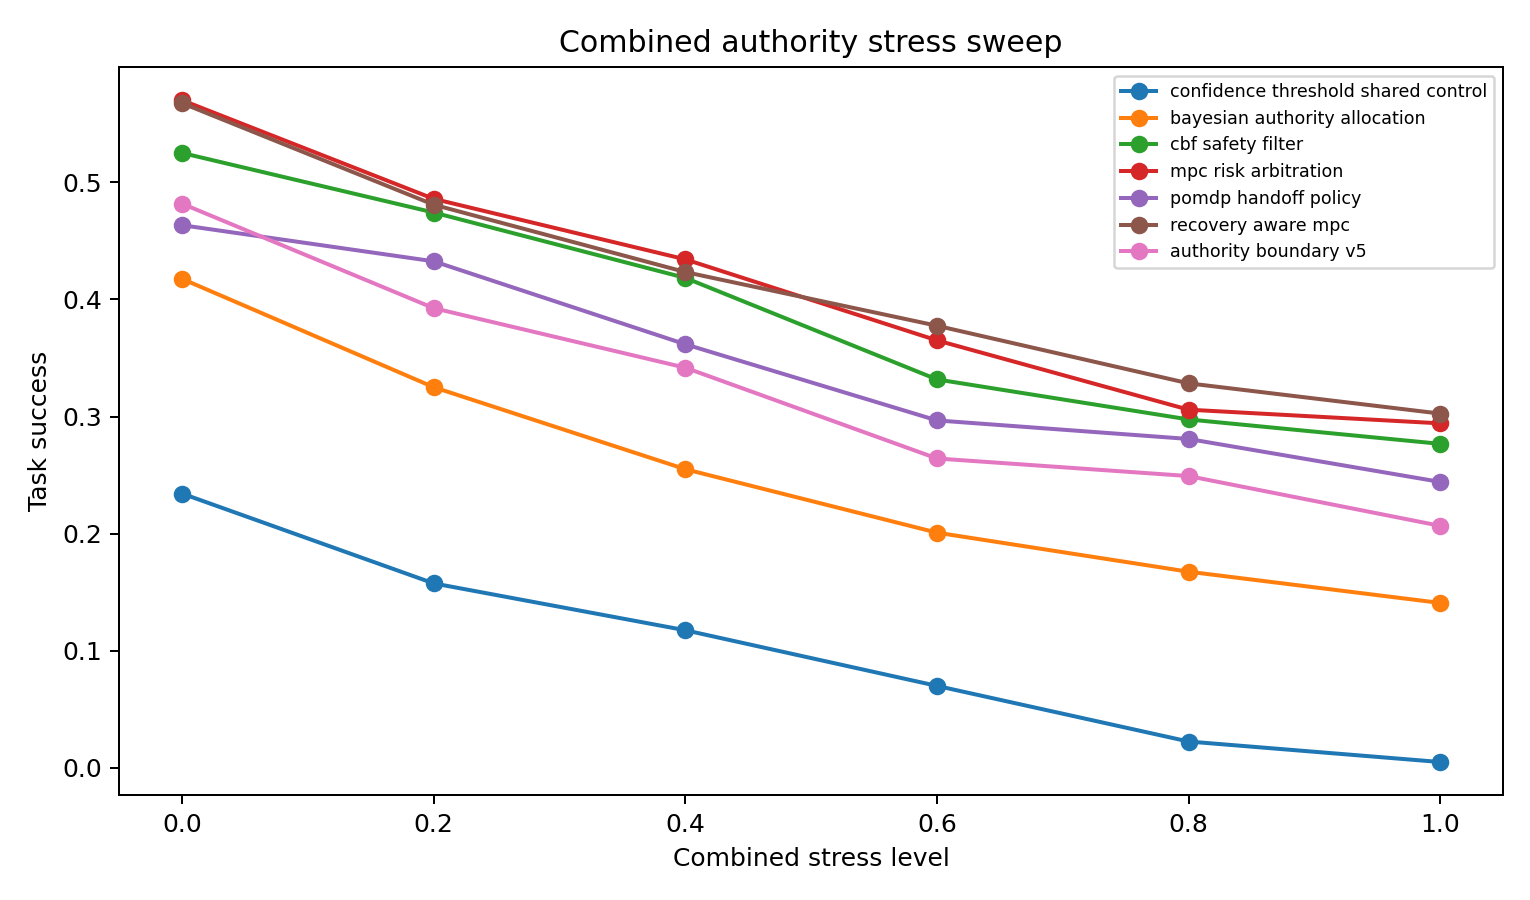
\includegraphics[width=0.95\linewidth]{authority_boundary_stress_sweep_v5.png}\caption{Task success under combined authority stress.}\end{figure}

\begin{figure}[t]\centering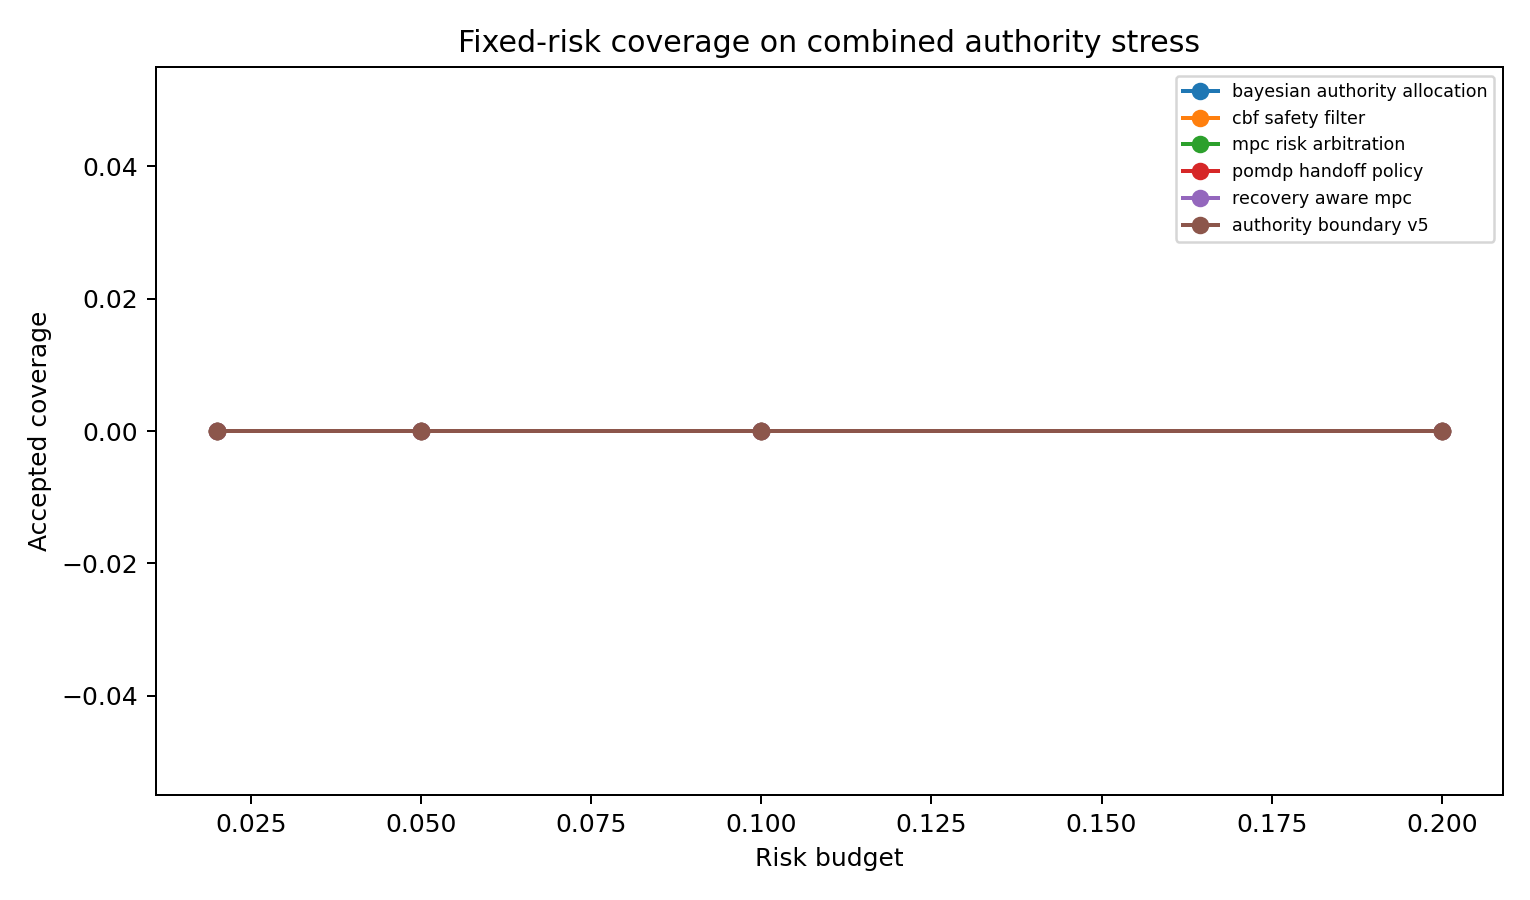
\includegraphics[width=0.95\linewidth]{authority_boundary_fixed_risk_v5.png}\caption{Fixed-risk coverage on combined authority stress.}\end{figure}

\begin{figure}[t]\centering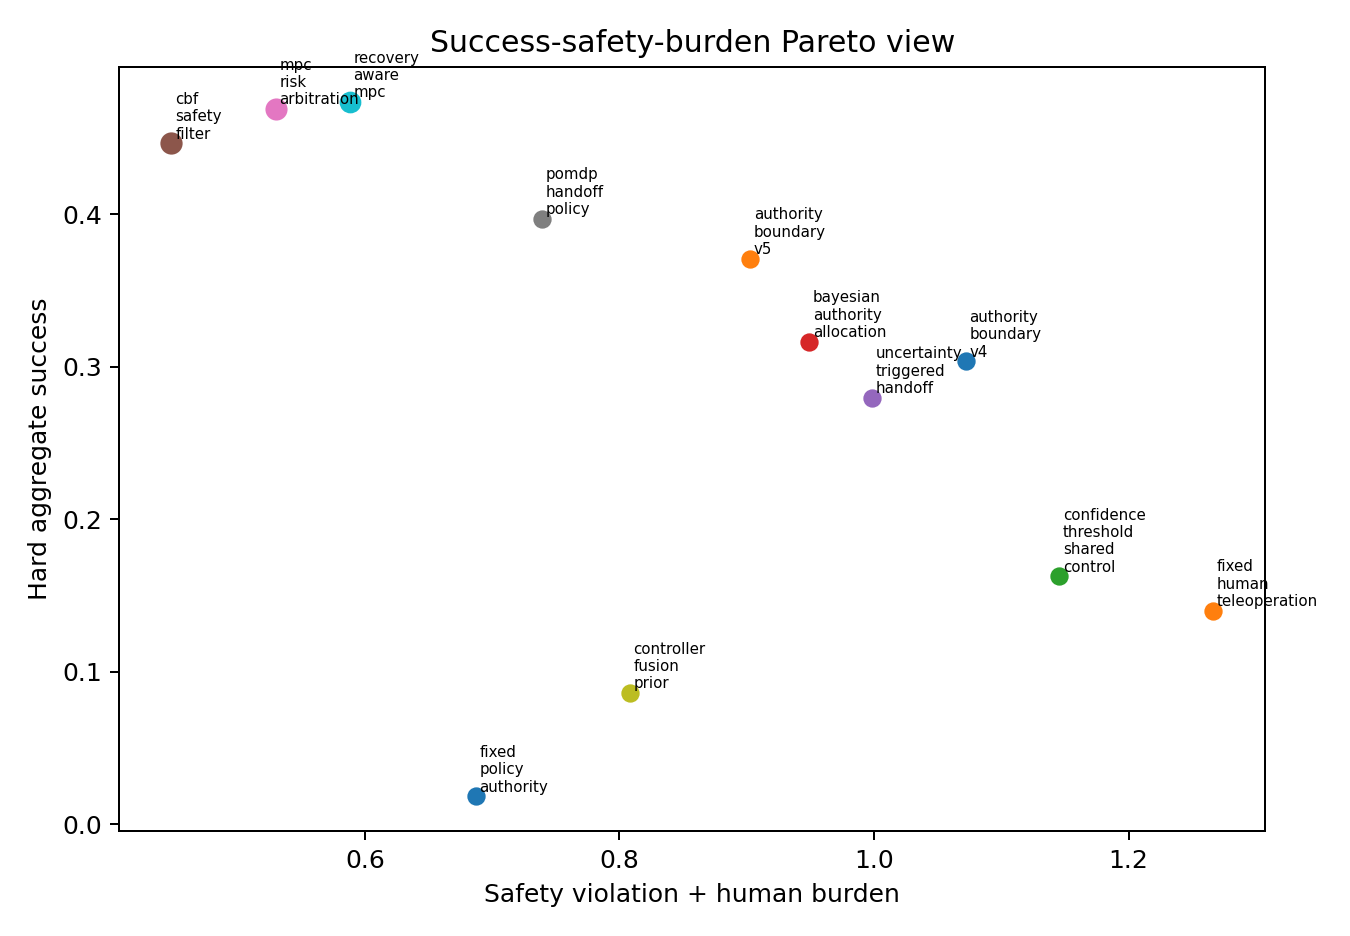
\includegraphics[width=0.75\linewidth]{authority_boundary_pareto_v5.png}\caption{Hard-aggregate Pareto view for success, safety, burden, and utility.}\end{figure}

\section{Reproducibility, Artifact Location, and Ethics}

All rows were generated locally on CPU with deterministic seeds. The final numbered PDF is copied only to Downloads. No Desktop PDF is produced. This paper should not be submitted as ICLR main without real robot or accepted high-fidelity validation.

\clearpage

\appendix

\section{Raw Summary Extract}

\begin{center}
\tiny
\begin{longtable}{rp{0.84\linewidth}}
\caption{Wrapped extract from results/summary.txt.}\label{tab:summaryextract}\\
\toprule
Line & Summary extract\\
\midrule
\endfirsthead
\caption[]{Wrapped extract from results/summary.txt. (continued)}\\
\toprule
Line & Summary extract\\
\midrule
\endhead
1 & Paper 90 control\_authority\_boundaries v5 expanded audit\\
2 & Terminal recommendation: KILL\_ARCHIVE\\
3 & ICLR main ready: no\\
4 & Reason: expanded CPU-only control-authority audit adds stronger CBF, MPC, POMDP, recovery-aware, uncertainty, ablation, stress, and fixed-risk tests, but no real robot or accepted high-fidelity deployment benchmark evidence exists\\
5 & Main rollout rows: 199680\\
6 & Dataset summary rows: 15360\\
7 & Main seed-metric rows: 1040\\
8 & Main metric rows: 1248\\
9 & Main pairwise rows: 672\\
10 & Hard aggregate seed rows: 130\\
11 & Hard aggregate metric rows: 156\\
12 & Hard aggregate pairwise rows: 84\\
13 & Ablation rollout rows: 33600\\
14 & Ablation seed rows: 200\\
15 & Ablation metric rows: 20\\
16 & Stress raw rows: 302400\\
17 & Stress seed rows: 2520\\
18 & Stress metric rows: 252\\
19 & Fixed-risk raw rows: 69120\\
20 & Fixed-risk seed rows: 480\\
21 & Fixed-risk metric rows: 48\\
22 & Fixed-risk pairwise rows: 200\\
23 & Negative cases: 24\\
25 & Frozen hard-aggregate gate:\\
26 & best\_success\_reference=recovery\_aware\_mpc\\
27 & safest\_reference=cbf\_safety\_filter\\
28 & lowest\_burden\_reference=fixed\_policy\_authority\\
29 & lowest\_regret\_reference=mpc\_risk\_arbitration\\
30 & best\_utility\_reference=cbf\_safety\_filter\\
31 & proposal\_success=0.37096\\
32 & best\_success=0.47370\\
33 & proposal\_safety=0.22734\\
34 & safest\_safety=0.15404\\
35 & proposal\_burden=0.67510\\
36 & lowest\_burden=0.26831\\
37 & proposal\_regret=0.31249\\
38 & lowest\_regret=0.24285\\
39 & proposal\_utility=-0.09423\\
40 & best\_utility=0.16009\\
41 & paired\_success\_lower95=-0.12094\\
42 & paired\_safety\_upper95=0.08260\\
43 & main\_gate=False\\
44 & mechanism\_gate=False\\
45 & mechanism\_best\_removed=safety\_only\_boundary\\
46 & stress\_gate=False\\
47 & stress\_dominated\_by=cbf\_safety\_filter\\
48 & fixed\_risk\_gate=False\\
49 & scope\_gate=False\\
50 & low\_signal\_high\_risk\_shift: v5\_coverage=0.00000, best\_feasible\_coverage=0.00000, v5\_success=0.00000, best\_feasible\_success=0.00000, v5\_safety=0.00000, best\_feasible\_safety=0.00000 | combined\_authority\_stress: v5\_coverage=0.00000, \\
52 & Hard aggregate metrics:\\
53 & fixed\_policy\_authority task\_success=0.01823 safety=0.41862 burden=0.26831 regret=0.63259 late=0.53935 churn=0.31974 utility=-0.60137\\
54 & fixed\_human\_teleoperation task\_success=0.13997 safety=0.26654 burden=0.99980 regret=0.40281 late=0.40063 churn=0.30982 utility=-0.48033\\
55 & confidence\_threshold\_shared\_control task\_success=0.16250 safety=0.29635 burden=0.84908 regret=0.43979 late=0.38356 churn=0.46987 utility=-0.46111\\
56 & bayesian\_authority\_allocation task\_success=0.31654 safety=0.24987 burden=0.69923 regret=0.33283 late=0.33014 churn=0.40970 utility=-0.18359\\
57 & uncertainty\_triggered\_handoff task\_success=0.27982 safety=0.22617 burden=0.77185 regret=0.35436 late=0.32311 churn=0.49993 utility=-0.24252\\
58 & cbf\_safety\_filter task\_success=0.44648 safety=0.15404 burden=0.29398 regret=0.26412 late=0.28285 churn=0.33990 utility=0.16009\\
59 & mpc\_risk\_arbitration task\_success=0.46901 safety=0.19062 burden=0.33930 regret=0.24285 late=0.26731 churn=0.35020 utility=0.15433\\
60 & pomdp\_handoff\_policy task\_success=0.39714 safety=0.21615 burden=0.52321 regret=0.28029 late=0.29211 churn=0.38970 utility=-0.00731\\
61 & controller\_fusion\_prior task\_success=0.08607 safety=0.37031 burden=0.43762 regret=0.56034 late=0.38481 churn=0.43978 utility=-0.50860\\
62 & recovery\_aware\_mpc task\_success=0.47370 safety=0.20156 burden=0.38643 regret=0.25674 late=0.26338 churn=0.35974 utility=0.13605\\
63 & authority\_boundary\_v4 task\_success=0.30365 safety=0.24310 burden=0.82884 regret=0.34824 late=0.30946 churn=0.43980 utility=-0.22875\\
64 & authority\_boundary\_v5 task\_success=0.37096 safety=0.22734 burden=0.67510 regret=0.31249 late=0.29451 churn=0.41995 utility=-0.09423\\
65 & oracle\_authority\_assignment task\_success=0.55287 safety=0.12747 burden=0.38300 regret=0.18831 late=0.24876 churn=0.32992 utility=0.29331\\
67 & Key paired hard-aggregate differences:\\
68 & v5\_minus\_authority\_boundary\_v4 authority\_regret: mean=-0.03575 ci95=0.00040 lower95=-0.03615 upper95=-0.03535\\
69 & v5\_minus\_authority\_boundary\_v4 human\_burden: mean=-0.15374 ci95=0.00046 lower95=-0.15420 upper95=-0.15328\\
70 & v5\_minus\_authority\_boundary\_v4 robust\_utility: mean=0.13452 ci95=0.02027 lower95=0.11425 upper95=0.15479\\
71 & v5\_minus\_authority\_boundary\_v4 safety\_violation: mean=-0.01576 ci95=0.01420 lower95=-0.02996 upper95=-0.00155\\
72 & v5\_minus\_authority\_boundary\_v4 task\_success: mean=0.06732 ci95=0.01615 lower95=0.05117 upper95=0.08347\\
73 & v5\_minus\_cbf\_safety\_filter authority\_regret: mean=0.04838 ci95=0.00041 lower95=0.04797 upper95=0.04879\\
74 & v5\_minus\_cbf\_safety\_filter human\_burden: mean=0.38112 ci95=0.00053 lower95=0.38059 upper95=0.38166\\
75 & v5\_minus\_cbf\_safety\_filter robust\_utility: mean=-0.25432 ci95=0.01008 lower95=-0.26440 upper95=-0.24425\\
76 & v5\_minus\_cbf\_safety\_filter safety\_violation: mean=0.07331 ci95=0.00930 lower95=0.06401 upper95=0.08260\\
77 & v5\_minus\_cbf\_safety\_filter task\_success: mean=-0.07552 ci95=0.01190 lower95=-0.08742 upper95=-0.06362\\
78 & v5\_minus\_recovery\_aware\_mpc authority\_regret: mean=0.05575 ci95=0.00027 lower95=0.05549 upper95=0.05602\\
79 & v5\_minus\_recovery\_aware\_mpc human\_burden: mean=0.28867 ci95=0.00057 lower95=0.28809 upper95=0.28924\\
80 & v5\_minus\_recovery\_aware\_mpc robust\_utility: mean=-0.23028 ci95=0.01716 lower95=-0.24744 upper95=-0.21312\\
81 & v5\_minus\_recovery\_aware\_mpc safety\_violation: mean=0.02578 ci95=0.01572 lower95=0.01006 upper95=0.04150\\
82 & v5\_minus\_recovery\_aware\_mpc task\_success: mean=-0.10273 ci95=0.01820 lower95=-0.12094 upper95=-0.08453\\
84 & Ablation utility:\\
85 & confidence\_only\_boundary success=0.12202 safety=0.31012 burden=0.84354 utility=-0.52941\\
86 & full\_authority\_boundary\_v5 success=0.31190 safety=0.22024 burden=0.70912 utility=-0.17729\\
87 & minus\_boundary\_uncertainty success=0.30000 safety=0.28214 burden=0.68175 utility=-0.23573\\
88 & minus\_consequence\_risk\_model success=0.25417 safety=0.31667 burden=0.68326 utility=-0.30783\\
89 & minus\_handoff\_hysteresis success=0.33452 safety=0.23869 burden=0.72934 utility=-0.19666\\
90 & minus\_human\_burden\_model success=0.33809 safety=0.26131 burden=0.89816 utility=-0.22508\\
91 & minus\_intent\_ambiguity\_gate success=0.37024 safety=0.25655 burden=0.51801 utility=-0.07057\\
92 & minus\_recovery\_feasibility success=0.29762 safety=0.24524 burden=0.68956 utility=-0.21815\\
93 & mpc\_only\_boundary success=0.41845 safety=0.20536 burden=0.38331 utility=0.06065\\
94 & safety\_only\_boundary success=0.40357 safety=0.16845 burden=0.32781 utility=0.07944\\
96 & Maximum combined stress:\\
97 & confidence\_threshold\_shared\_control task\_success=0.00500 safety=0.40667 burden=0.99530 utility=-0.81291\\
98 & bayesian\_authority\_allocation task\_success=0.14083 safety=0.31917 burden=0.86569 utility=-0.53318\\
99 & cbf\_safety\_filter task\_success=0.27667 safety=0.21667 burden=0.46016 utility=-0.17817\\
100 & mpc\_risk\_arbitration task\_success=0.29417 safety=0.25000 burden=0.50502 utility=-0.18696\\
101 & pomdp\_handoff\_policy task\_success=0.24417 safety=0.27833 burden=0.68907 utility=-0.32896\\
102 & recovery\_aware\_mpc task\_success=0.30250 safety=0.27583 burden=0.55264 utility=-0.21091\\
103 & authority\_boundary\_v5 task\_success=0.20667 safety=0.28667 burden=0.84131 utility=-0.42587\\
105 & Fixed-risk budget 0.05:\\
106 & combined\_authority\_stress authority\_boundary\_v5 coverage=0.00000 accepted\_success=0.00000 accepted\_safety=0.00000 accepted\_regret=0.00000\\
107 & combined\_authority\_stress bayesian\_authority\_allocation coverage=0.00000 accepted\_success=0.00000 accepted\_safety=0.00000 accepted\_regret=0.00000\\
108 & combined\_authority\_stress cbf\_safety\_filter coverage=0.00000 accepted\_success=0.00000 accepted\_safety=0.00000 accepted\_regret=0.00000\\
109 & combined\_authority\_stress mpc\_risk\_arbitration coverage=0.00000 accepted\_success=0.00000 accepted\_safety=0.00000 accepted\_regret=0.00000\\
110 & combined\_authority\_stress pomdp\_handoff\_policy coverage=0.00000 accepted\_success=0.00000 accepted\_safety=0.00000 accepted\_regret=0.00000\\
111 & combined\_authority\_stress recovery\_aware\_mpc coverage=0.00000 accepted\_success=0.00000 accepted\_safety=0.00000 accepted\_regret=0.00000\\
112 & low\_signal\_high\_risk\_shift authority\_boundary\_v5 coverage=0.00000 accepted\_success=0.00000 accepted\_safety=0.00000 accepted\_regret=0.00000\\
113 & low\_signal\_high\_risk\_shift bayesian\_authority\_allocation coverage=0.00000 accepted\_success=0.00000 accepted\_safety=0.00000 accepted\_regret=0.00000\\
114 & low\_signal\_high\_risk\_shift cbf\_safety\_filter coverage=0.00000 accepted\_success=0.00000 accepted\_safety=0.00000 accepted\_regret=0.00000\\
115 & low\_signal\_high\_risk\_shift mpc\_risk\_arbitration coverage=0.00000 accepted\_success=0.00000 accepted\_safety=0.00000 accepted\_regret=0.00000\\
116 & low\_signal\_high\_risk\_shift pomdp\_handoff\_policy coverage=0.00000 accepted\_success=0.00000 accepted\_safety=0.00000 accepted\_regret=0.00000\\
117 & low\_signal\_high\_risk\_shift recovery\_aware\_mpc coverage=0.00000 accepted\_success=0.00000 accepted\_safety=0.00000 accepted\_regret=0.00000\\
119 & Negative cases: 24\\
120 & terminal=KILL\_ARCHIVE\\
\bottomrule
\end{longtable}
\normalsize
\end{center}

\bibliographystyle{iclr2026_conference}

\bibliography{references}

\end{document}
